\documentclass[a4paper,10pt,twoside,twocolumn,final]{JICS_LaTexGuidelines} %These are the only supported options
\RequirePackage{geometry} % Provides margin and dimmentions finetuning.
\geometry{ % DO NOT MODIFY
	top=1.5 cm,
	left=1.7cm,
	right=1.7cm,
	textheight=25.3cm,
	headsep=0.25cm,
	columnsep=0.6cm,
	footskip=1.2cm
}

\usepackage{cite}
\usepackage{pgfkeys}
\usepackage{multirow}

\pgfkeys{
    /erro_pmos_current/.is family,
    /erro_pmos_current,
    short/.initial = 0.42,
    long/.initial = 2.28,
    icemos/.initial = 9.49
}

\pgfkeys{
    /erro_nmos_current/.is family,
    /erro_nmos_current,
    short/.initial = 1.81,
    long/.initial = 2.19,
    icemos/.initial = 1.11
}

\pgfkeys{
    /erro_pmos_gm/.is family,
    /erro_pmos_gm,
    short/.initial = 1.52,
    long/.initial = 7.65,
    icemos/.initial = 5.95
}

\pgfkeys{
    /erro_nmos_gm/.is family,
    /erro_nmos_gm,
    short/.initial = 2.87,
    long/.initial = 2.69,
    icemos/.initial = 2.46
}

\begin{document}
	% TITLE
\title{A Design-Oriented Open-Source Cryogenic SPICE Model for Sky130 CMOS with Automated Calibration Using Experimental 4 K Data}
	% AUTHORS AND AFFILIATIONS
\author{Edson Alves da Silva\textsuperscript1, Lucas Stucchi-Zucchi\textsuperscript2, Marcelo A. Pavanello\textsuperscript3, Jose Alexandre Diniz\textsuperscript4, and Francisco A. Brito-Filho\textsuperscript5\\\vspace{1.2em}\small%
\textsuperscript1Edson Alves da Silva, Engineering Department, F.U. of the Semiarid Region (UFERSA), Mossoró, Brazil\\%
\textsuperscript{2,4}Lucas Stucchi-Zucchi and Jose Alexandre Diniz, Electrical Engineering Department, University of Campinas (UNICAMP), Campinas, Brazil\\%
\textsuperscript3Marcelo A. Pavanello, Electrical Engineering Department, Centro Universitário FEI, Sao Bernardo do Campo, Brazil\\%
\textsuperscript5Francisco A. Brito-Filho, Engineering Department, F.U. of the Semiarid Region (UFERSA), Caraubas, Brazil\\%
e-mail: edson.silva17274@alunos.ufersa.edu.br
}
%
	% HEADERS AND FOOTERS
\markboth{Journal of Integrated Circuits and Systems, vol. XX, n. XX, 2026}%
{SILVA et al.: Design-Oriented Open-Source Cryogenic SPICE Model for Sky130}%
\renewcommand*\footnoterule{}%
\footnotetext{Digital Object Identifier 10.29292/jics.vXXiX.X}%
\maketitle
	% ABSTRACT SECTION
\begin{abstract}
	Cryogenic compact models are essential for the design of CMOS interface circuits operating near 4 K, particularly in emerging applications such as quantum computing control and readout electronics. However, accurate model extraction at cryogenic temperatures often depends on costly commercial tools or labor-intensive manual calibration flows. This work presents a fully automated methodology for generating cryogenic BSIM4 models for the open-source Sky130 technology using experimental transistor measurements from the NIST 4 K dataset. The proposed flow combines physics-based parameter initialization using SEKV-E with iterative differential-evolution optimization driven by NGSPICE simulations, enabling scalable geometry-specific model generation without manual tuning. The calibration is design-oriented, prioritizing moderate and strong inversion regions, where most analog and mixed-signal circuits operate. Experimental validation is performed using transfer characteristics, output characteristics, transconductance, and $g_m/I_D$ metrics for NMOS and PMOS devices with multiple channel lengths. In the strong inversion region, mean relative current errors of \pgfkeysvalueof{/erro_pmos_current/short}\% and \pgfkeysvalueof{/erro_pmos_current/long}\% were achieved for PMOS devices, while NMOS devices reached \pgfkeysvalueof{/erro_nmos_current/short}\% and \pgfkeysvalueof{/erro_nmos_current/long}\%.
\end{abstract}
	% INDEX TERMS SECTION
\begin{indexterms}
	Cryogenic CMOS; BSIM4; Sky130; differential evolution; quantum computing.
\end{indexterms}
	% BODY SECTIONS
\section{Introduction}

Quantum computing platforms require electronic interfaces capable of operating at cryogenic temperatures, typically near 4 K, for qubit control and readout \cite{b1,b2,b3,b16}. In this context, Cryo-CMOS has become an important technology for improving scalability and reducing interconnection complexity.

At such temperatures, conventional CMOS models no longer accurately describe transistor behavior. Relevant deviations arise in threshold voltage, carrier mobility, and subthreshold response, directly affecting circuit performance \cite{b4}. Therefore, accurate compact models at 4 K are essential.

Recent studies introduced open-source calibration strategies for Sky130 CMOS at 4 K \cite{b5,b6,b7}. Although effective, generating calibrated models for multiple geometries still requires considerable user intervention.

This work presents a fully automated calibration methodology for geometry-specific cryogenic SPICE models in Sky130 CMOS, removing manual parameter initialization and enabling scalable model generation.

\section{Sky130 Cryogenic Modeling Challenges and Design-Oriented SPICE Model}

The Sky130 process design kit (PDK) has become one of the main open-source platforms for integrated circuit design, enabling reproducible research and reducing development costs \cite{b9,b10}. Its accessibility makes it attractive for emerging applications such as cryogenic control electronics for quantum computing systems.

However, at cryogenic temperatures (around 4 K), CMOS devices deviate significantly from room-temperature behavior. Experimental studies report threshold-voltage increase due to carrier freeze-out, mobility variations caused by the balance between reduced phonon scattering and increased impurity scattering, and non-ideal subthreshold behavior influenced by interface traps \cite{b4}. Additional effects such as the kink effect may also appear under specific bias conditions.

As a result, key characteristics such as drain current, transconductance, and output resistance are strongly modified, making the standard room-temperature BSIM models included in the Sky130 PDK insufficient for accurate 4 K circuit design.

To address this limitation, the proposed cryogenic model is based on the standard BSIM4 formulation \cite{b13,b14}, with selective recalibration of parameters rather than introducing a new compact model. This preserves compatibility with conventional design flows and industrial SPICE environments.

For physically consistent initialization, the SEKV-E methodology \cite{b12} is employed to estimate key device parameters before optimization. Similar strategies are used in recent cryogenic frameworks such as IceMOS \cite{b6}, since direct optimization without suitable starting points often leads to poor convergence or non-physical solutions.

Starting from this initialization, a fully automated optimization flow refines the BSIM4 parameters directly from experimental measurements, eliminating manual tuning and enabling scalable calibration across multiple geometries.

The proposed model is design-oriented, prioritizing accuracy in moderate and strong inversion regions, consistent with prior design-focused cryogenic modeling approaches \cite{b11}.

\section{Calibration Methodology}

The calibration process uses experimental data from the NIST Sky130 cryogenic dataset \cite{b15}, which provides transistor measurements at 4 K for different device geometries. These data are adopted as references for model fitting.

The proposed methodology follows three main stages: parameter initialization, grouped calibration, and model evaluation.

\subsection{Initial Parameter Estimation}

Initial values for key parameters, such as threshold voltage ($V_{th}$) and slope factor ($n$), are extracted from transfer characteristics using linear fitting in the subthreshold region. These estimates are further refined through the SEKV-E methodology \cite{b12}, providing physically meaningful starting points.

Temperature-dependent parameters (UTE, KT1, KT2, UA1, UB1) are fixed to zero during calibration, following common cryogenic modeling practices \cite{b4,b6}. This simplifies the model and improves optimization stability.

\subsection{Parameter Grouping Strategy}

Because BSIM4 contains many coupled parameters, calibration is divided into parameter groups according to physical impact. This reduces search complexity and improves convergence.

The groups target threshold behavior, mobility degradation, saturation effects, short-channel behavior, and additional PMOS corrections. Table~\ref{tab:param_groups} summarizes the adopted grouping.

\begin{table}[h]\tiny
	\centering
	\caption{Summary of parameter groups used in the calibration process}
	\label{tab:param_groups}
	\begin{tabular}{|c|l|}
		\hline
		\textbf{Group} & \textbf{Parameters} \\
		\hline
		Threshold / Transition & vth0, nfactor, voff, u0 \\
		\hline
		Body / Shape & k1, k2, ua, ub \\
		\hline
		Drive / Saturation & vsat, rdsw \\
		\hline
		Short-Channel / Output & a0, a1, a2, pclm \\
		\hline
		PMOS Additional & uc \\
		\hline
	\end{tabular}
\end{table}

This block-based strategy avoids simultaneous optimization of all variables, which often leads to poor convergence in nonlinear problems.

\subsection{Iterative Optimization}

Starting from the initialized set, parameters are refined through differential evolution. Candidate solutions are generated, inserted into the technology file, and simulated in NGSPICE through PySpice.

The optimizer minimizes the root-mean-square error (RMSE) between simulated and measured currents. Only current values above 1 pA are considered inside the cost function to reduce noise sensitivity and numerical issues in deep subthreshold.

Different calibration modes were investigated. The first used combined $I_D$--$V_G$ data at $V_{DS}=1.8\,\mathrm{V}$ and $0.1\,\mathrm{V}$, while the second used $I_D$--$V_G$ at $V_{DS}=1.8\,\mathrm{V}$ together with $I_D$--$V_D$ at $V_{GS}=1.8\,\mathrm{V}$. In both cases, higher weight was assigned to saturation-region data.

No single strategy was consistently optimal for all geometries. Therefore, the framework supports multiple calibration modes, allowing selection of the best fit for each device.

\subsection{Evaluation Criteria}

While the root-mean-square error (RMSE) serves as the cost function during the iterative optimization, the final model accuracy reported in Section IV is quantified using the Mean Absolute Percentage Error (MAPE). This provides a normalized relative error metric, allowing for a consistent evaluation of the model's performance across different current magnitudes and device geometries.

\section{Experimental Results and Validation}

The proposed cryogenic SPICE models were validated against measured 4 K data for multiple geometries. NMOS devices with $W=1.68\,\mu m$ and $L=0.15\,\mu m$, $1.00\,\mu m$, and PMOS devices with $W=0.42\,\mu m$ and $L=0.18\,\mu m$, $1.00\,\mu m$ were analyzed.

Model accuracy was evaluated through $I_D$--$V_G$, $I_D$--$V_D$, $g_m$, and $g_m/I_D$, covering weak, moderate, and strong inversion.

\subsection{Transfer Characteristics}

The PFET curves in Fig.~\ref{fig:IDVG_PFET}, obtained with $V_{SD}=1.8\,\mathrm{V}$, show excellent agreement in moderate and strong inversion, with larger deviations only in deep subthreshold. Mean current errors were \pgfkeysvalueof{/erro_pmos_current/short}\,\% and \pgfkeysvalueof{/erro_pmos_current/long}\,\% for $L=0.18\,\mu m$ and $1.00\,\mu m$, respectively.

\begin{figure}[h]
	\centering
	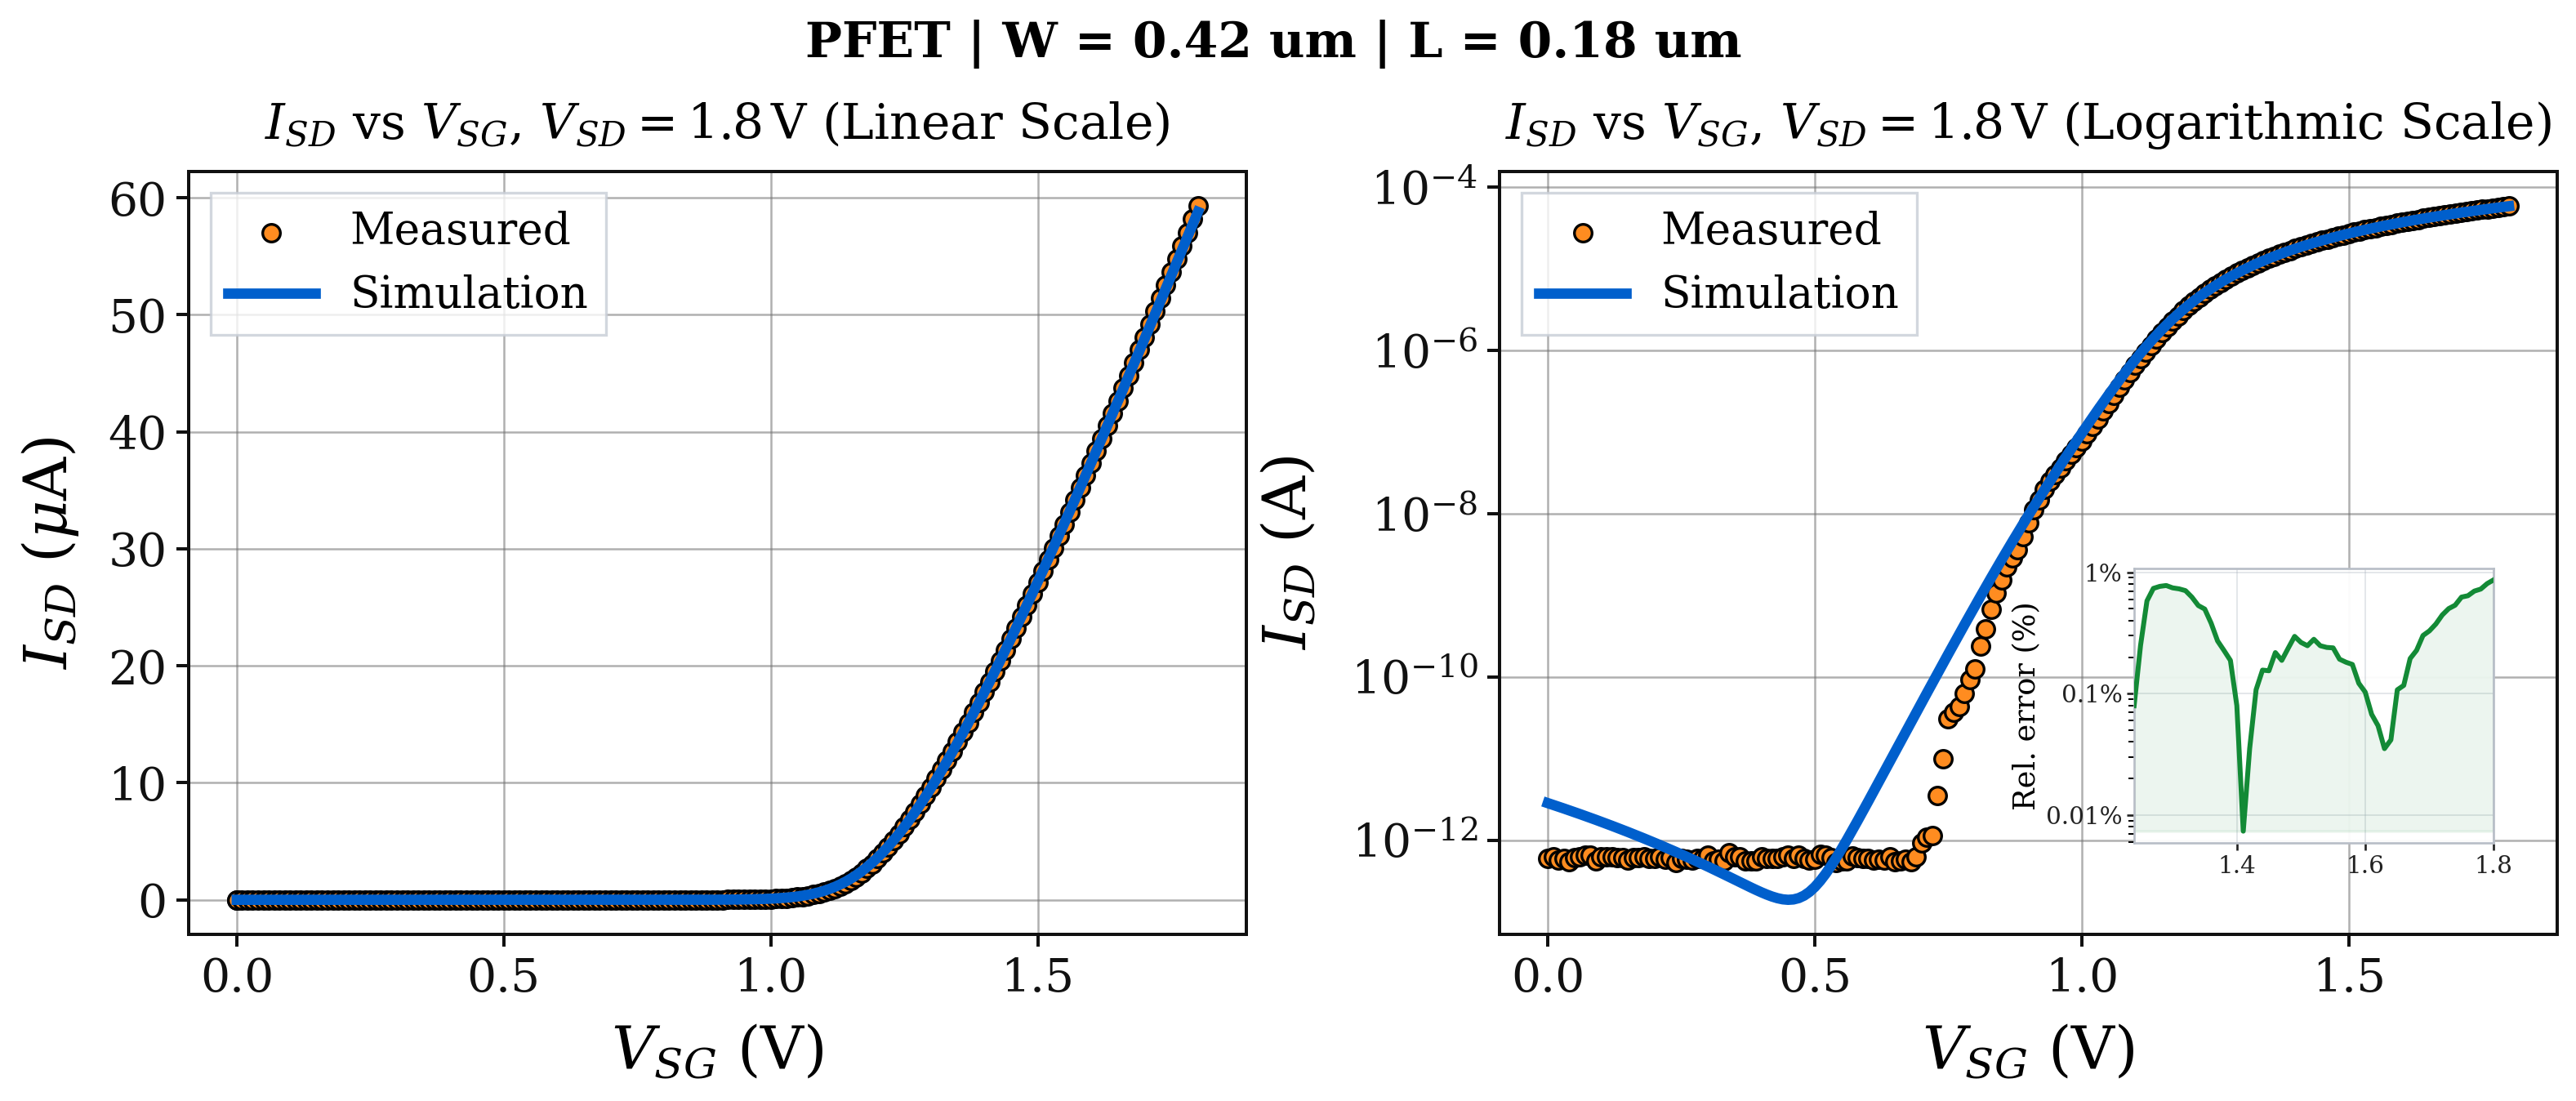
\includegraphics[width=\columnwidth]{fig/publication_pfet_saturacao_w0p42_l0p18.png}

	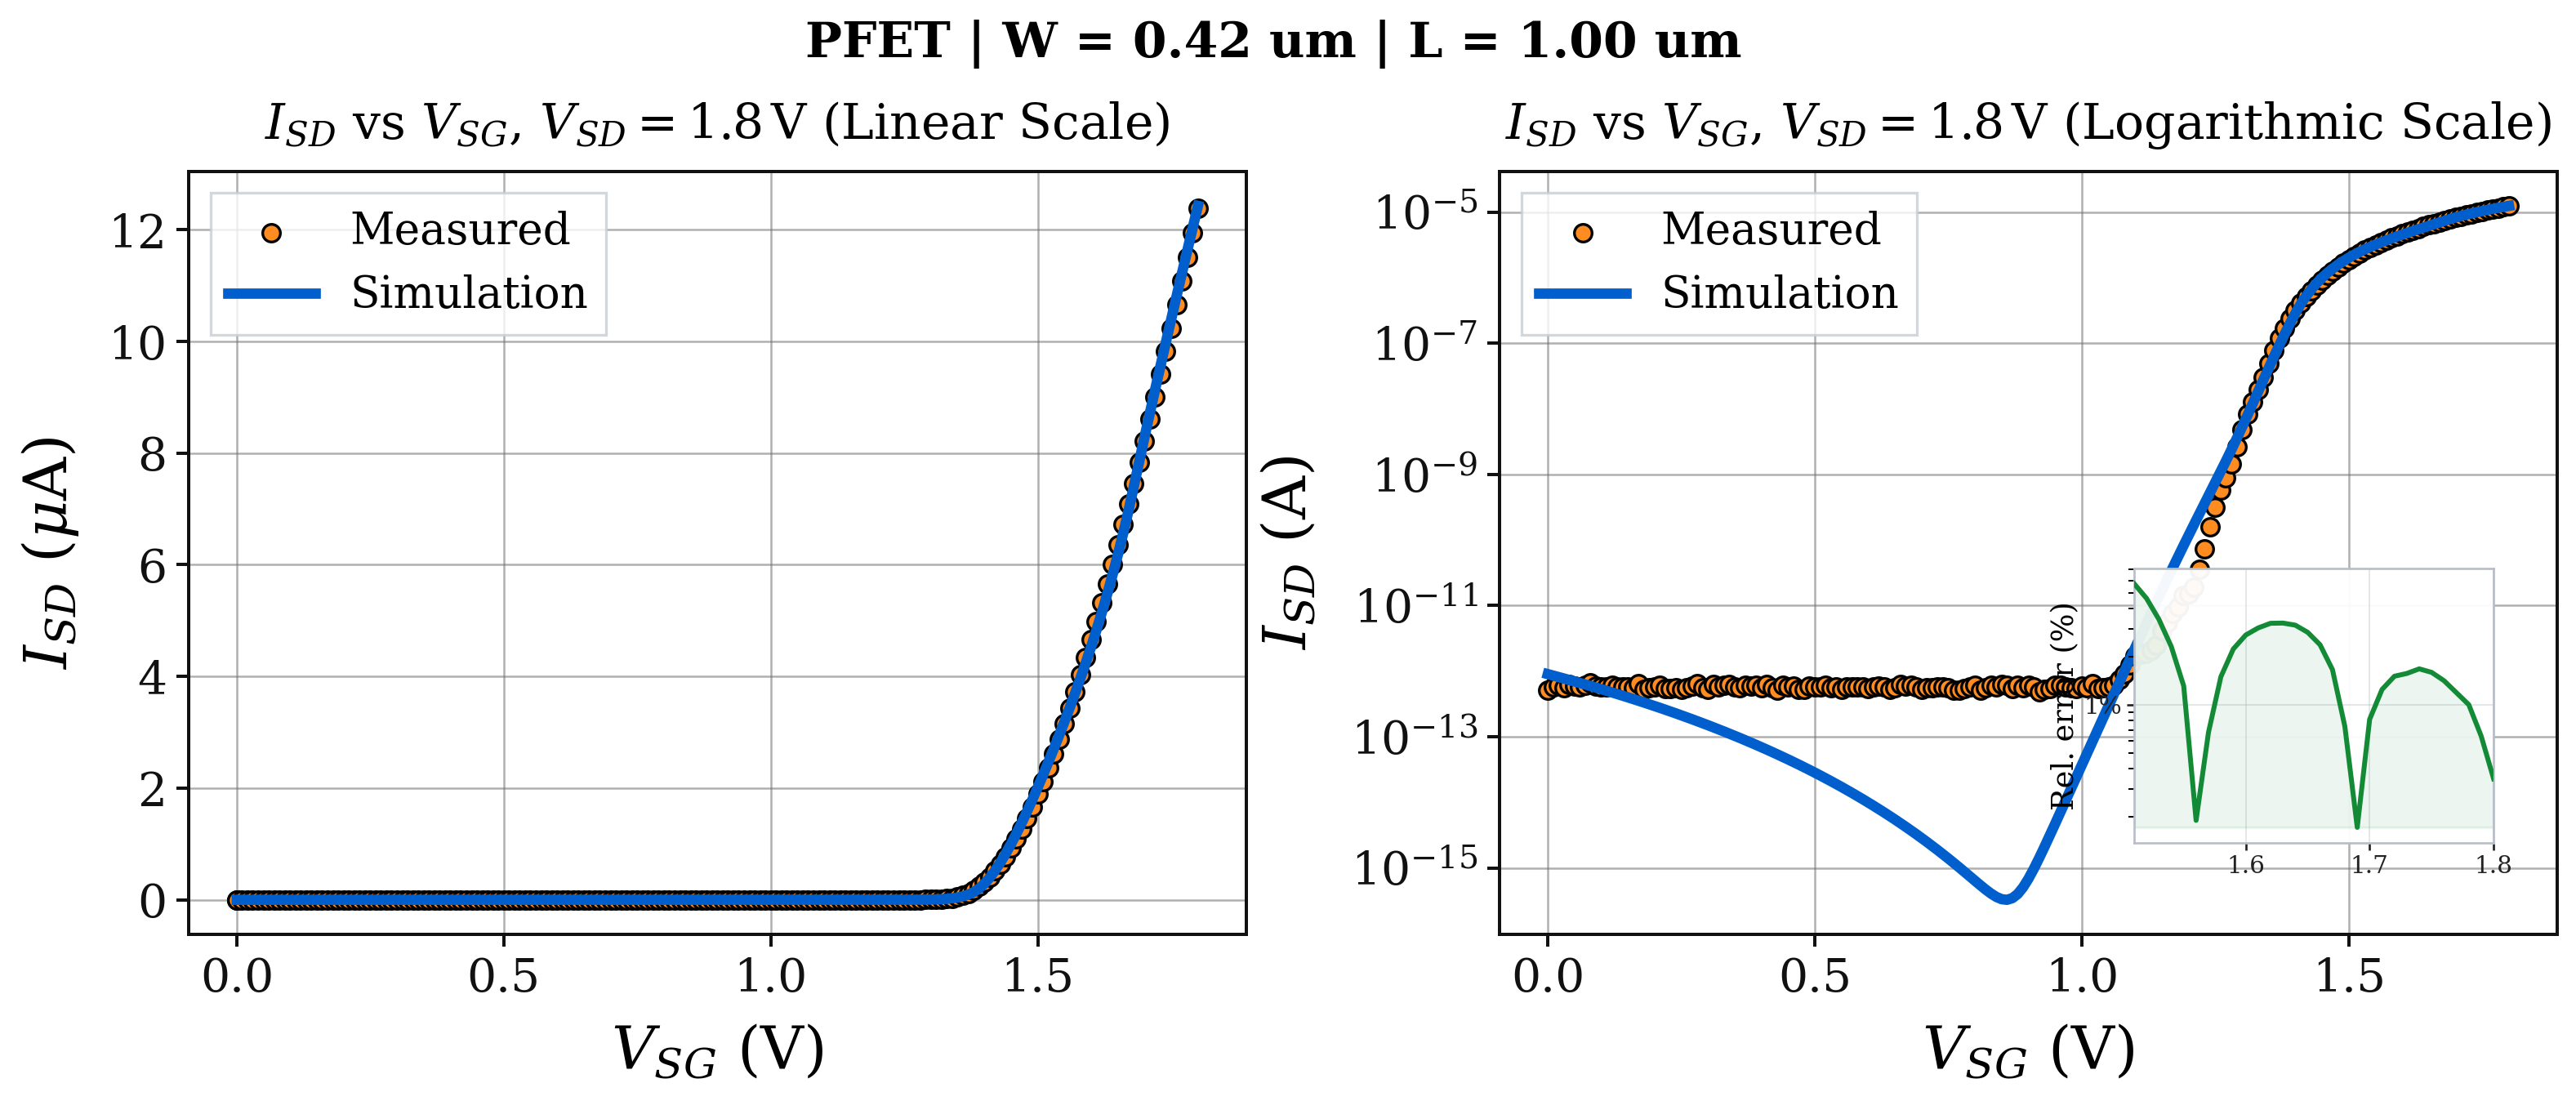
\includegraphics[width=\columnwidth]{fig/publication_pfet_saturacao_w0p42_l1.png}
	\caption{Measured and simulated transfer characteristics ($I_D$--$V_G$) for PFET devices at 4 K, shown in linear and logarithmic scales for different channel lengths.}
	\label{fig:IDVG_PFET}
\end{figure}

The NFET curves in Fig.~\ref{fig:IDVG_NFET}, obtained with $V_{DS}=1.8\,\mathrm{V}$, also show accurate fitting over the main operating region. Mean current errors were \pgfkeysvalueof{/erro_nmos_current/short}\,\% and \pgfkeysvalueof{/erro_nmos_current/long}\,\% for $L=0.15\,\mu m$ and $1.00\,\mu m$, respectively.

\begin{figure}[h]
	\centering
	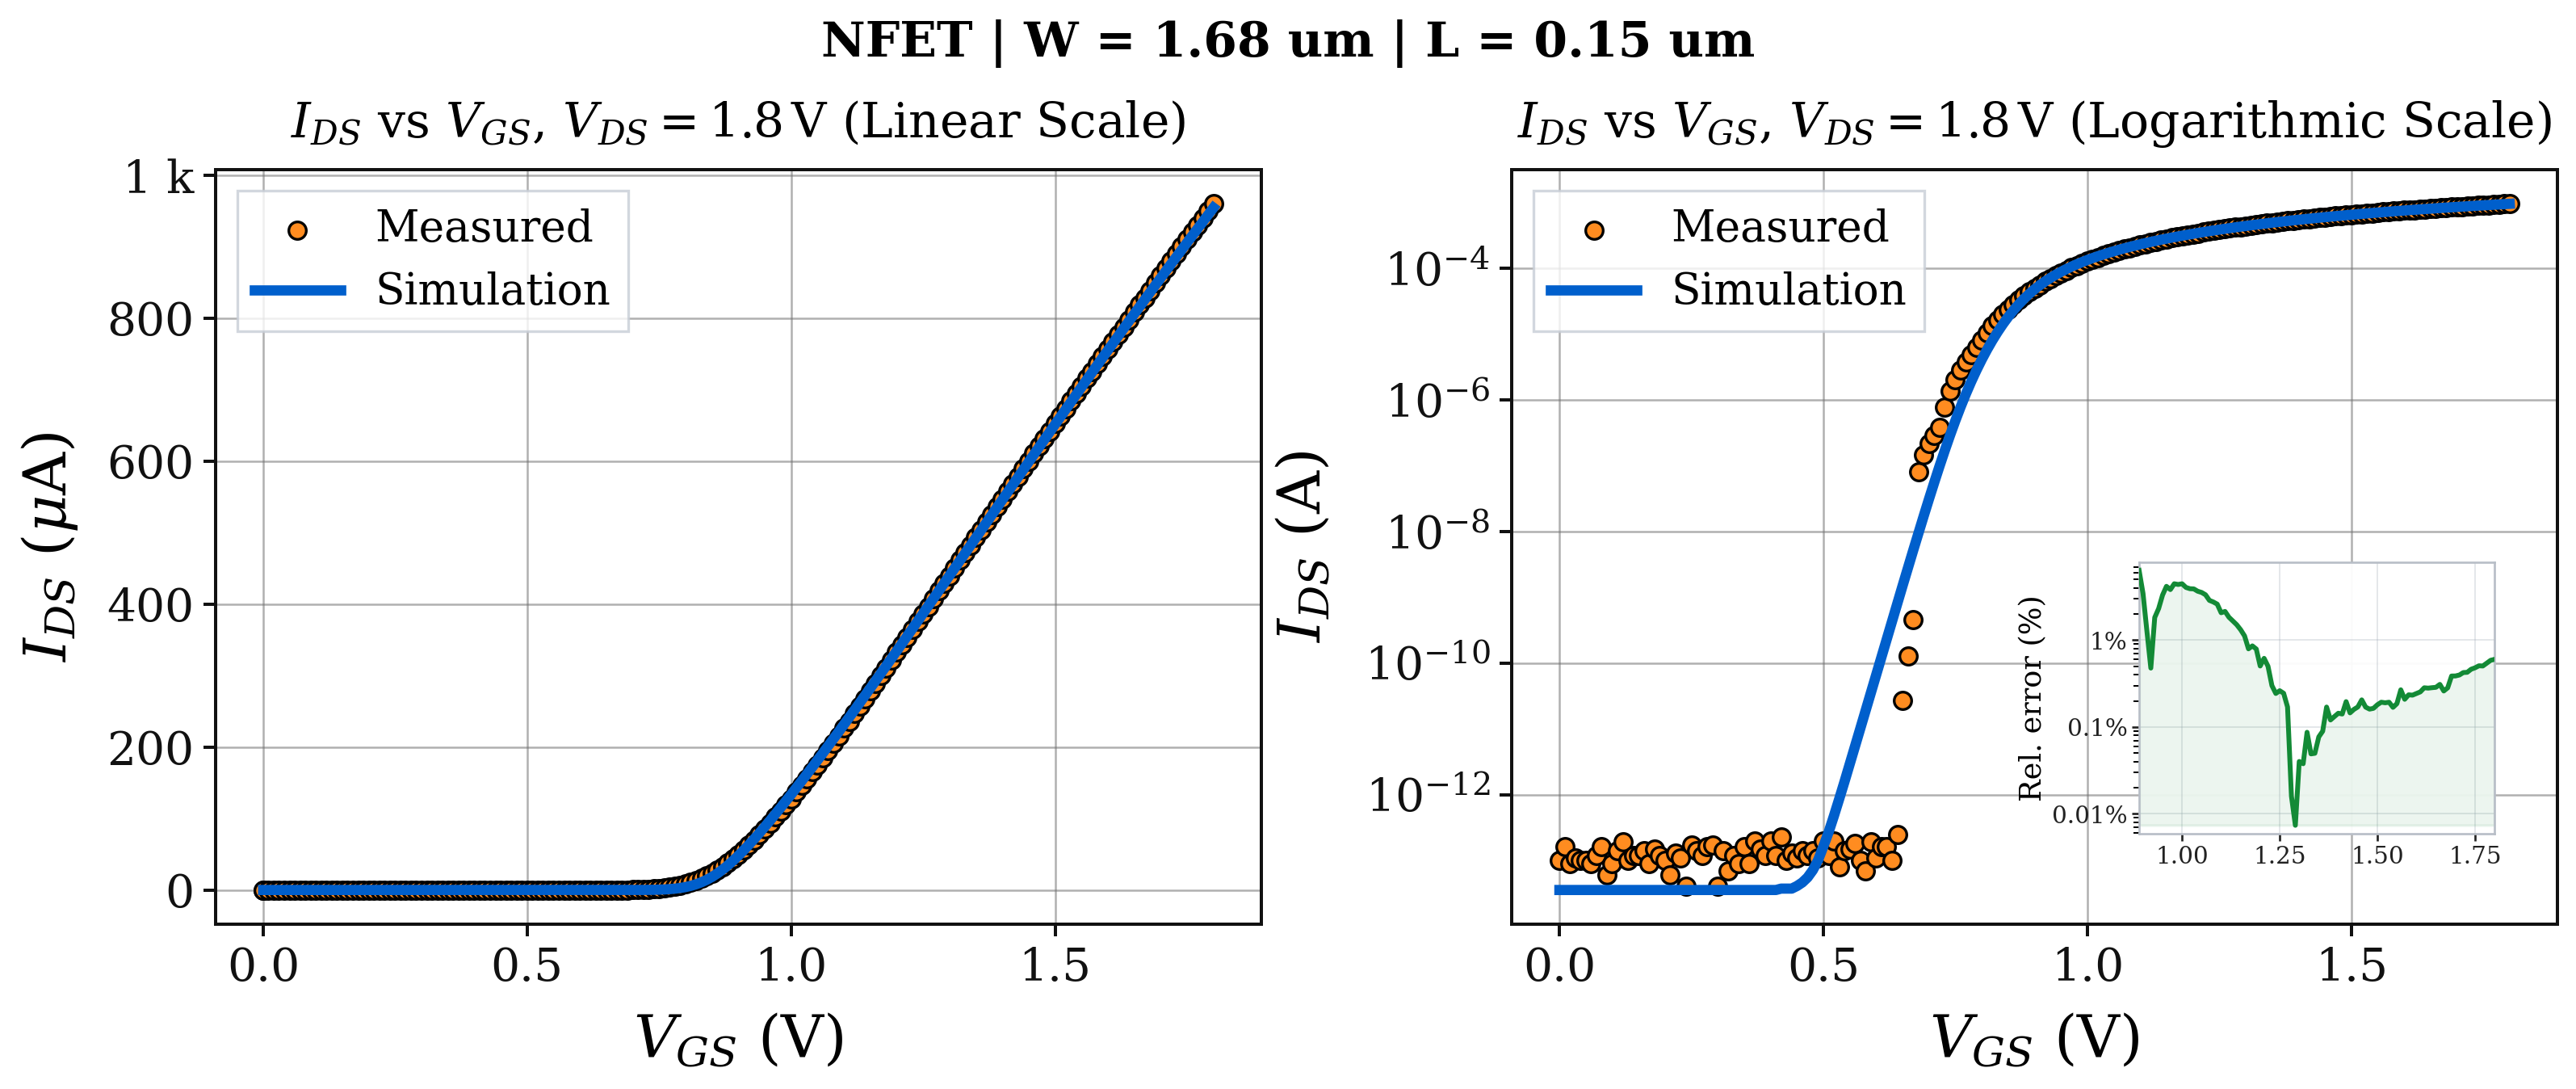
\includegraphics[width=\columnwidth]{fig/publication_nfet_saturacao_w1p68_l0p15.png}

	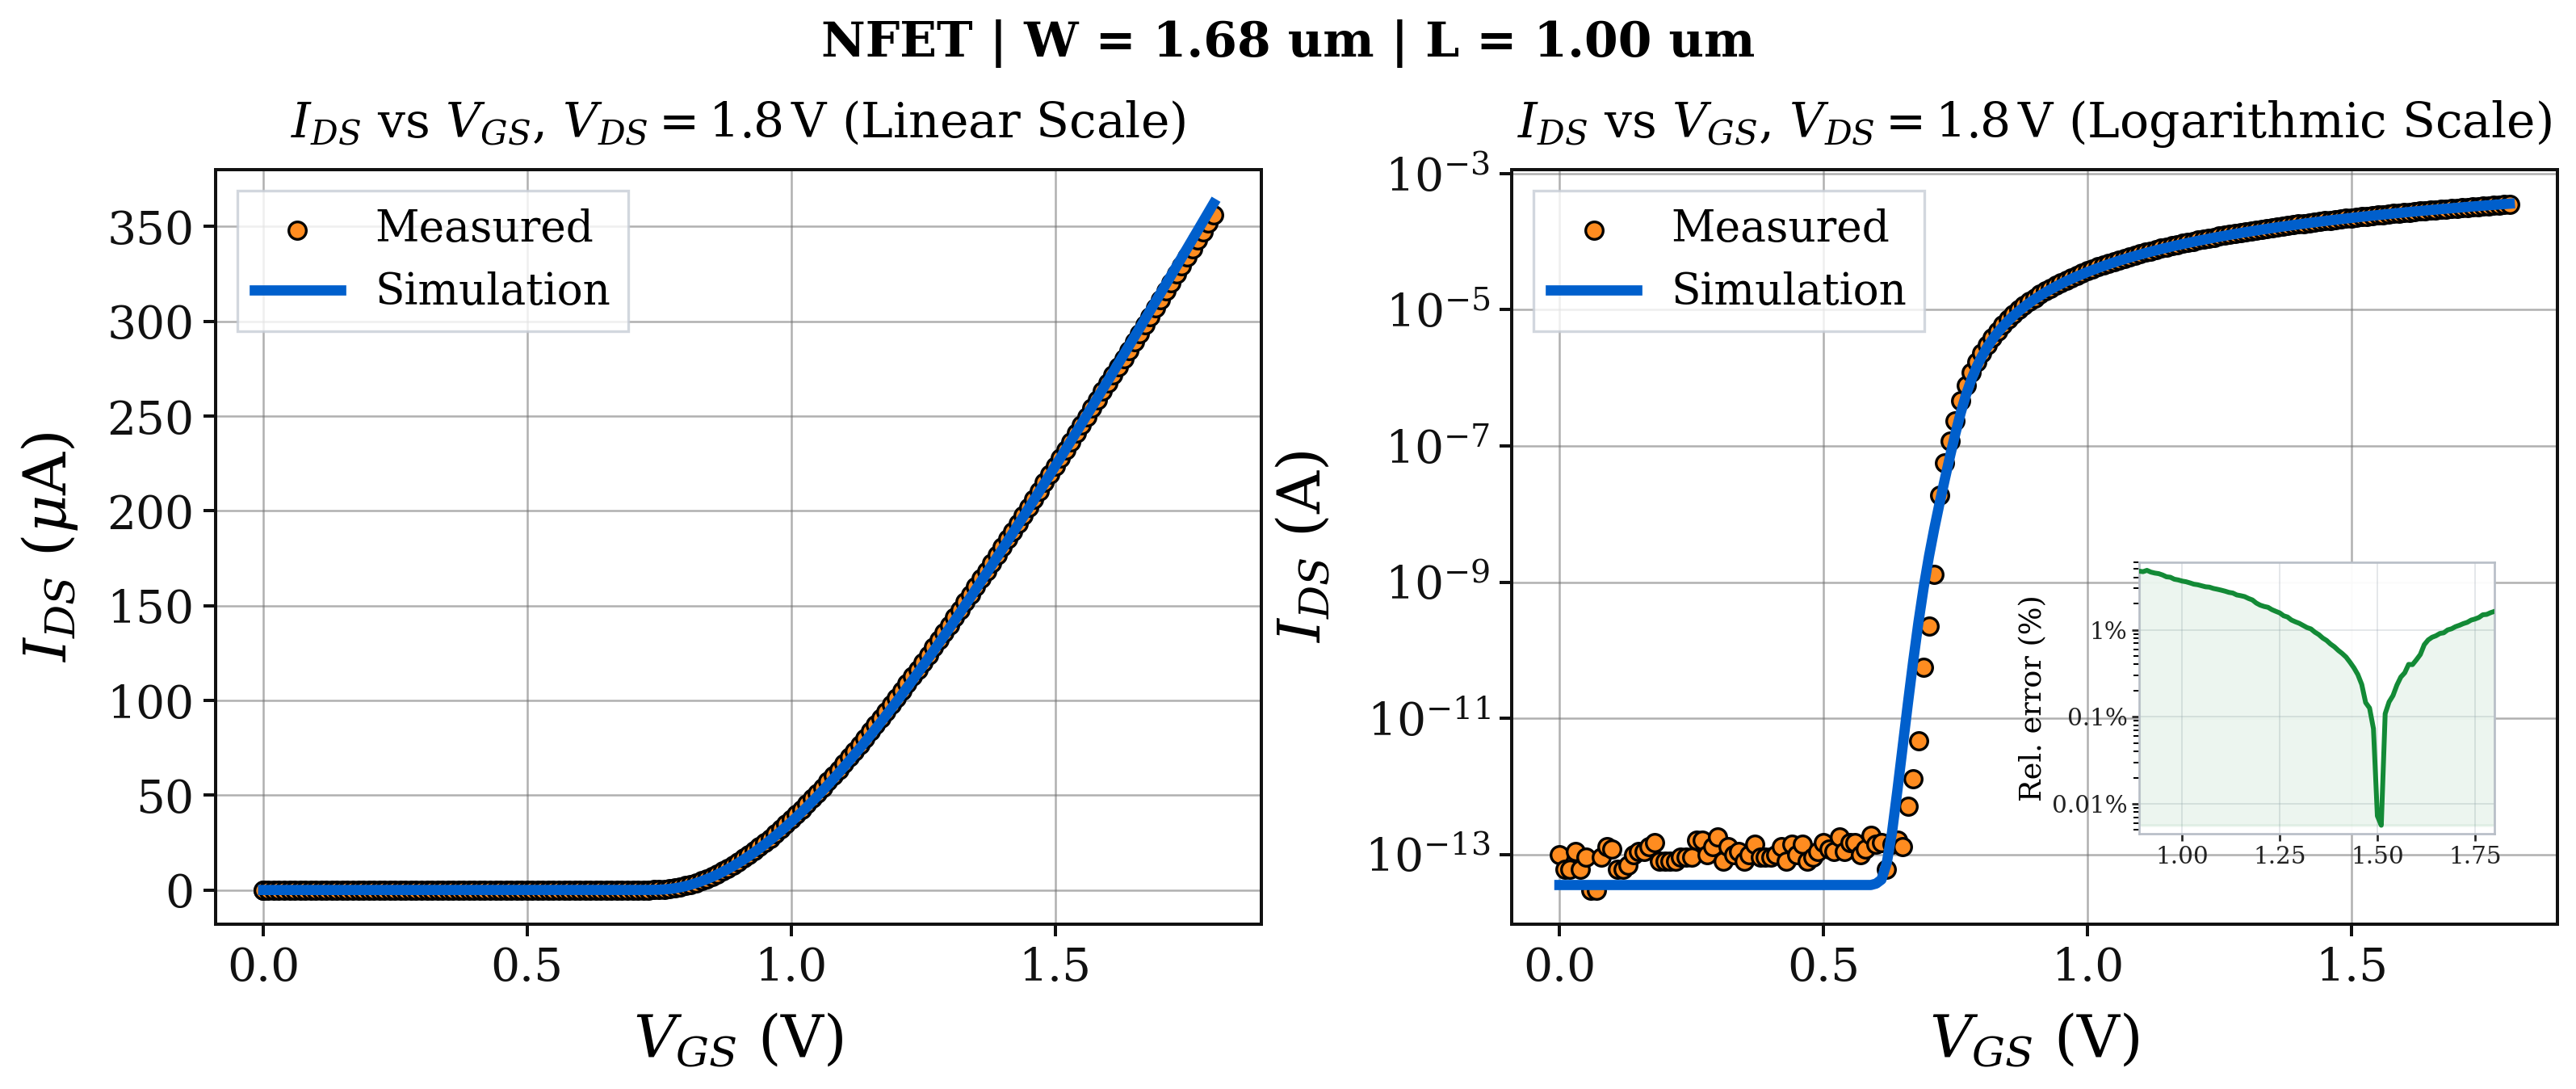
\includegraphics[width=\columnwidth]{fig/publication_nfet_saturacao_w1p68_l1.png}
	\caption{Measured and simulated transfer characteristics ($I_D$--$V_G$) for NFET devices at 4 K, shown in linear and logarithmic scales for different channel lengths.}
	\label{fig:IDVG_NFET}
\end{figure}

\subsection{Output Characteristics}

Fig.~\ref{fig:IDVD} compares measured and simulated $I_D$--$V_D$ curves for short-channel devices under several $V_{GS}$ values. Good agreement is observed in both linear and saturation regions.

\begin{figure}[h]
	\centering
	\begin{minipage}[t]{0.48\columnwidth}
		\centering
		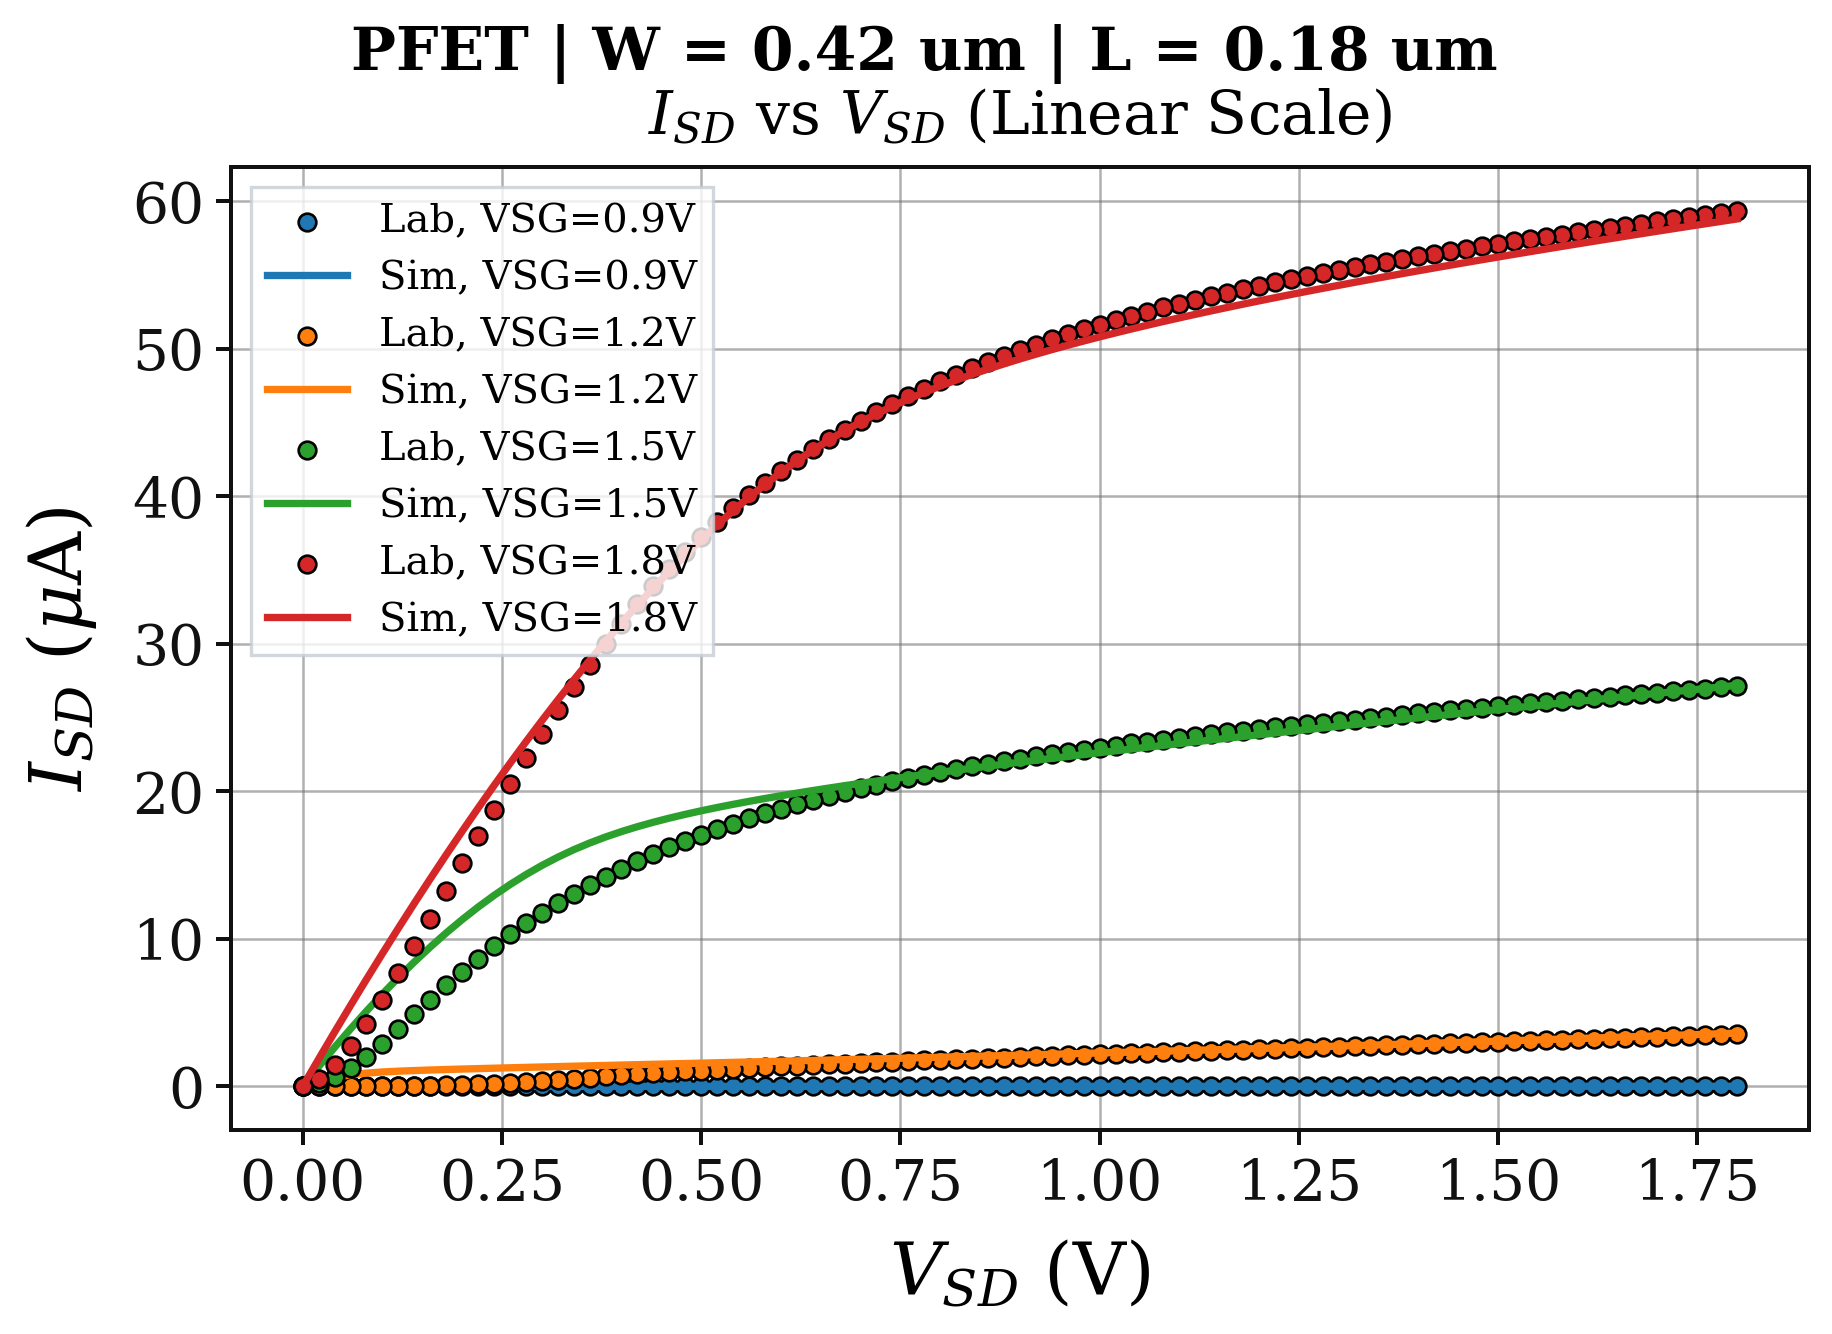
\includegraphics[width=\linewidth]{fig/publication_pfet_saturacao_w0p42_l0p18_idvd.png}\\
		{\tiny (a)}
	\end{minipage}
	\hfill
	\begin{minipage}[t]{0.48\columnwidth}
		\centering
		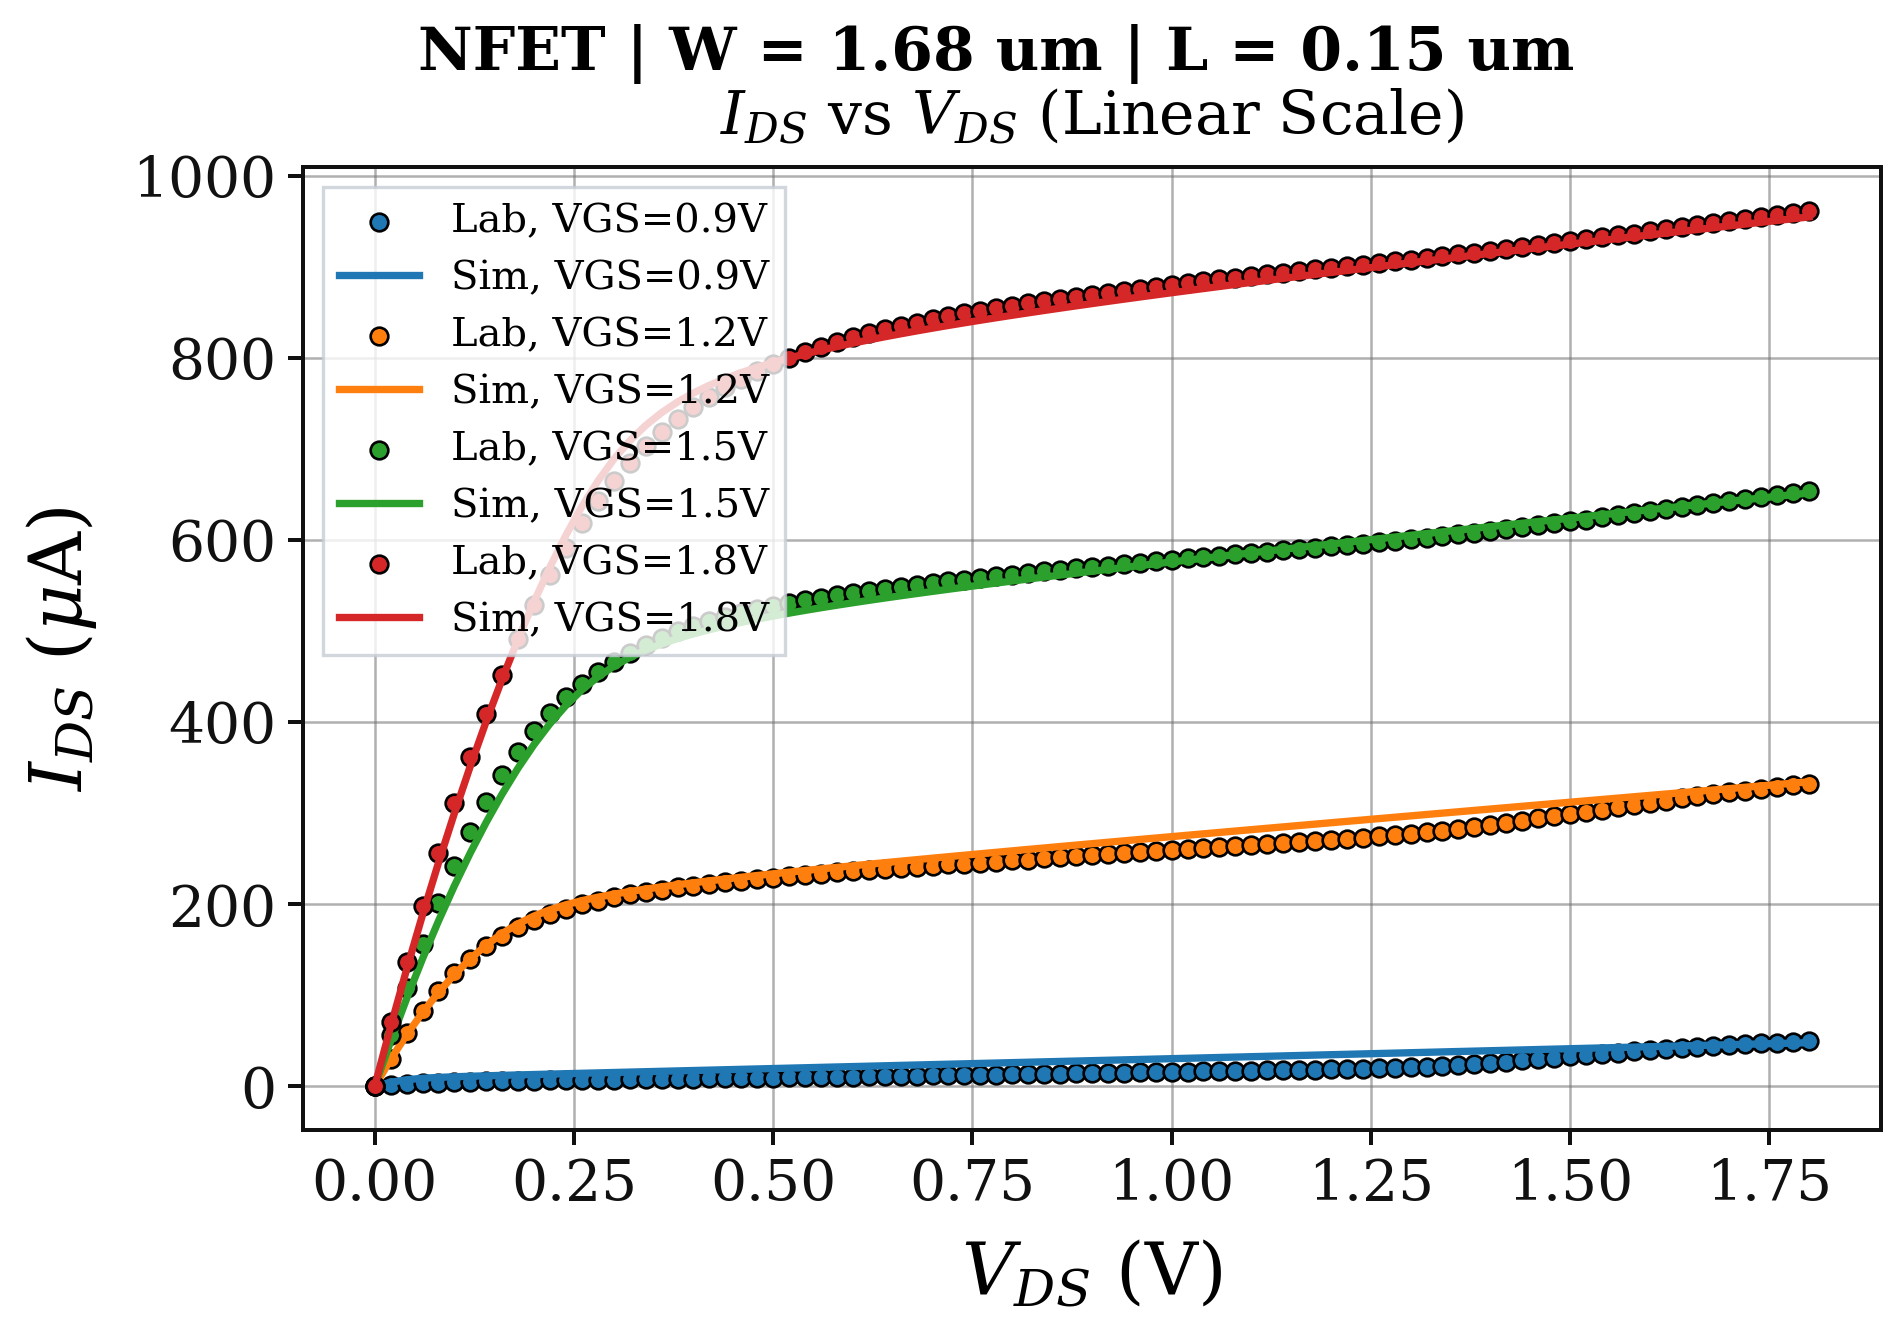
\includegraphics[width=\linewidth]{fig/publication_nfet_saturacao_w1p68_l0p15_idvd.png}\\
		{\tiny (b)}
	\end{minipage}
	\caption{Measured and simulated output characteristics ($I_D$--$V_D$) at 4 K for short-channel devices under different $V_{G}$ bias conditions: (a) PFET and (b) NFET.}
	\label{fig:IDVD}
\end{figure}

\subsection{Transconductance}

Fig.~\ref{fig:gmVG} shows that the calibrated models reproduce the measured $g_m$ behavior for $V_{SD}=1.8\,\mathrm{V}$ (or $V_{DS}=1.8\,\mathrm{V}$ for NFET), including the turn-on transition and peak values. Mean relative errors were \pgfkeysvalueof{/erro_pmos_gm/short}\,\%, \pgfkeysvalueof{/erro_pmos_gm/long}\,\%, \pgfkeysvalueof{/erro_nmos_gm/short}\,\%, and \pgfkeysvalueof{/erro_nmos_gm/long}\,\% for cases (a)--(d), respectively.

\begin{figure}[h]
	\centering
	\begin{minipage}[t]{0.48\columnwidth}
		\centering
		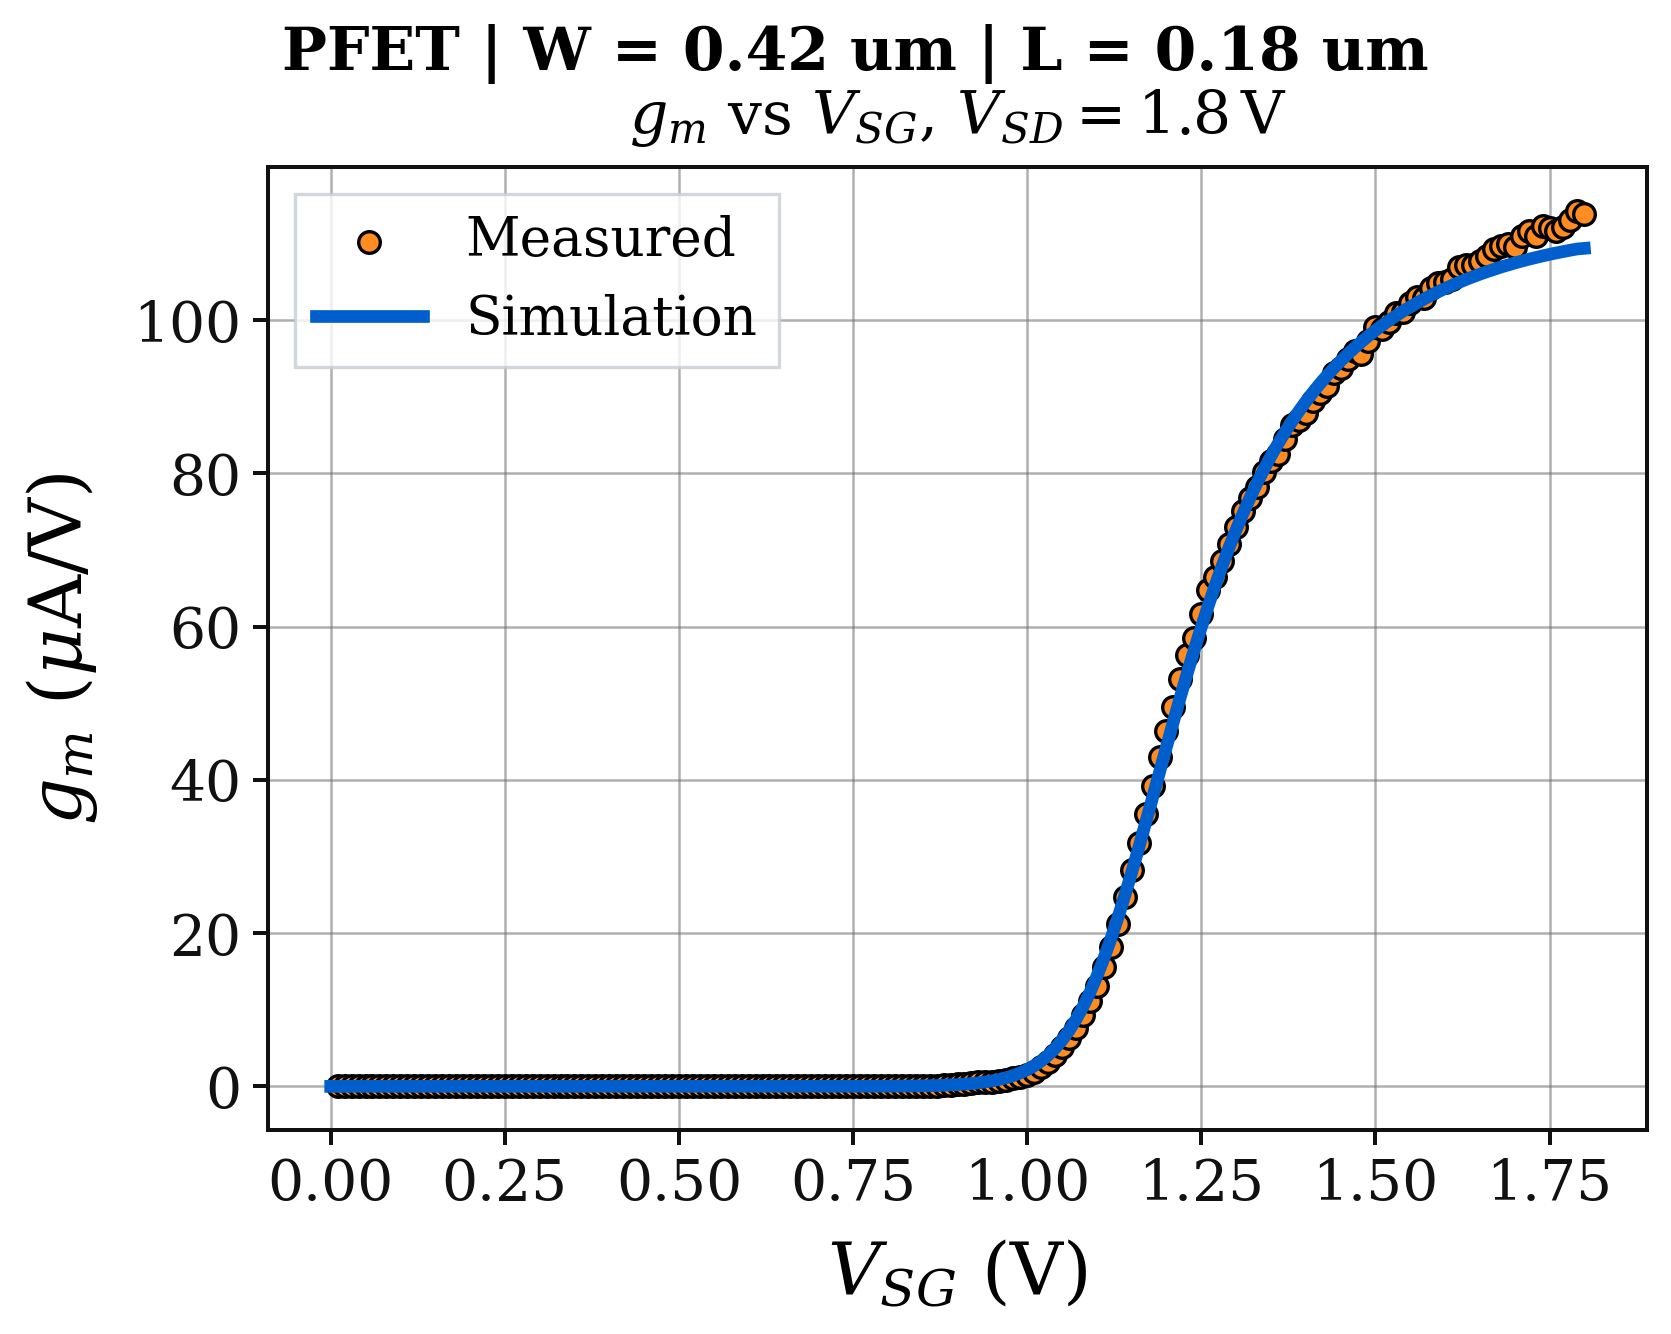
\includegraphics[width=\linewidth]{fig/publication_pfet_saturacao_w0p42_l0p18gmvg.png}\\
		{\tiny (a)}
	\end{minipage}
	\hfill
	\begin{minipage}[t]{0.48\columnwidth}
		\centering
		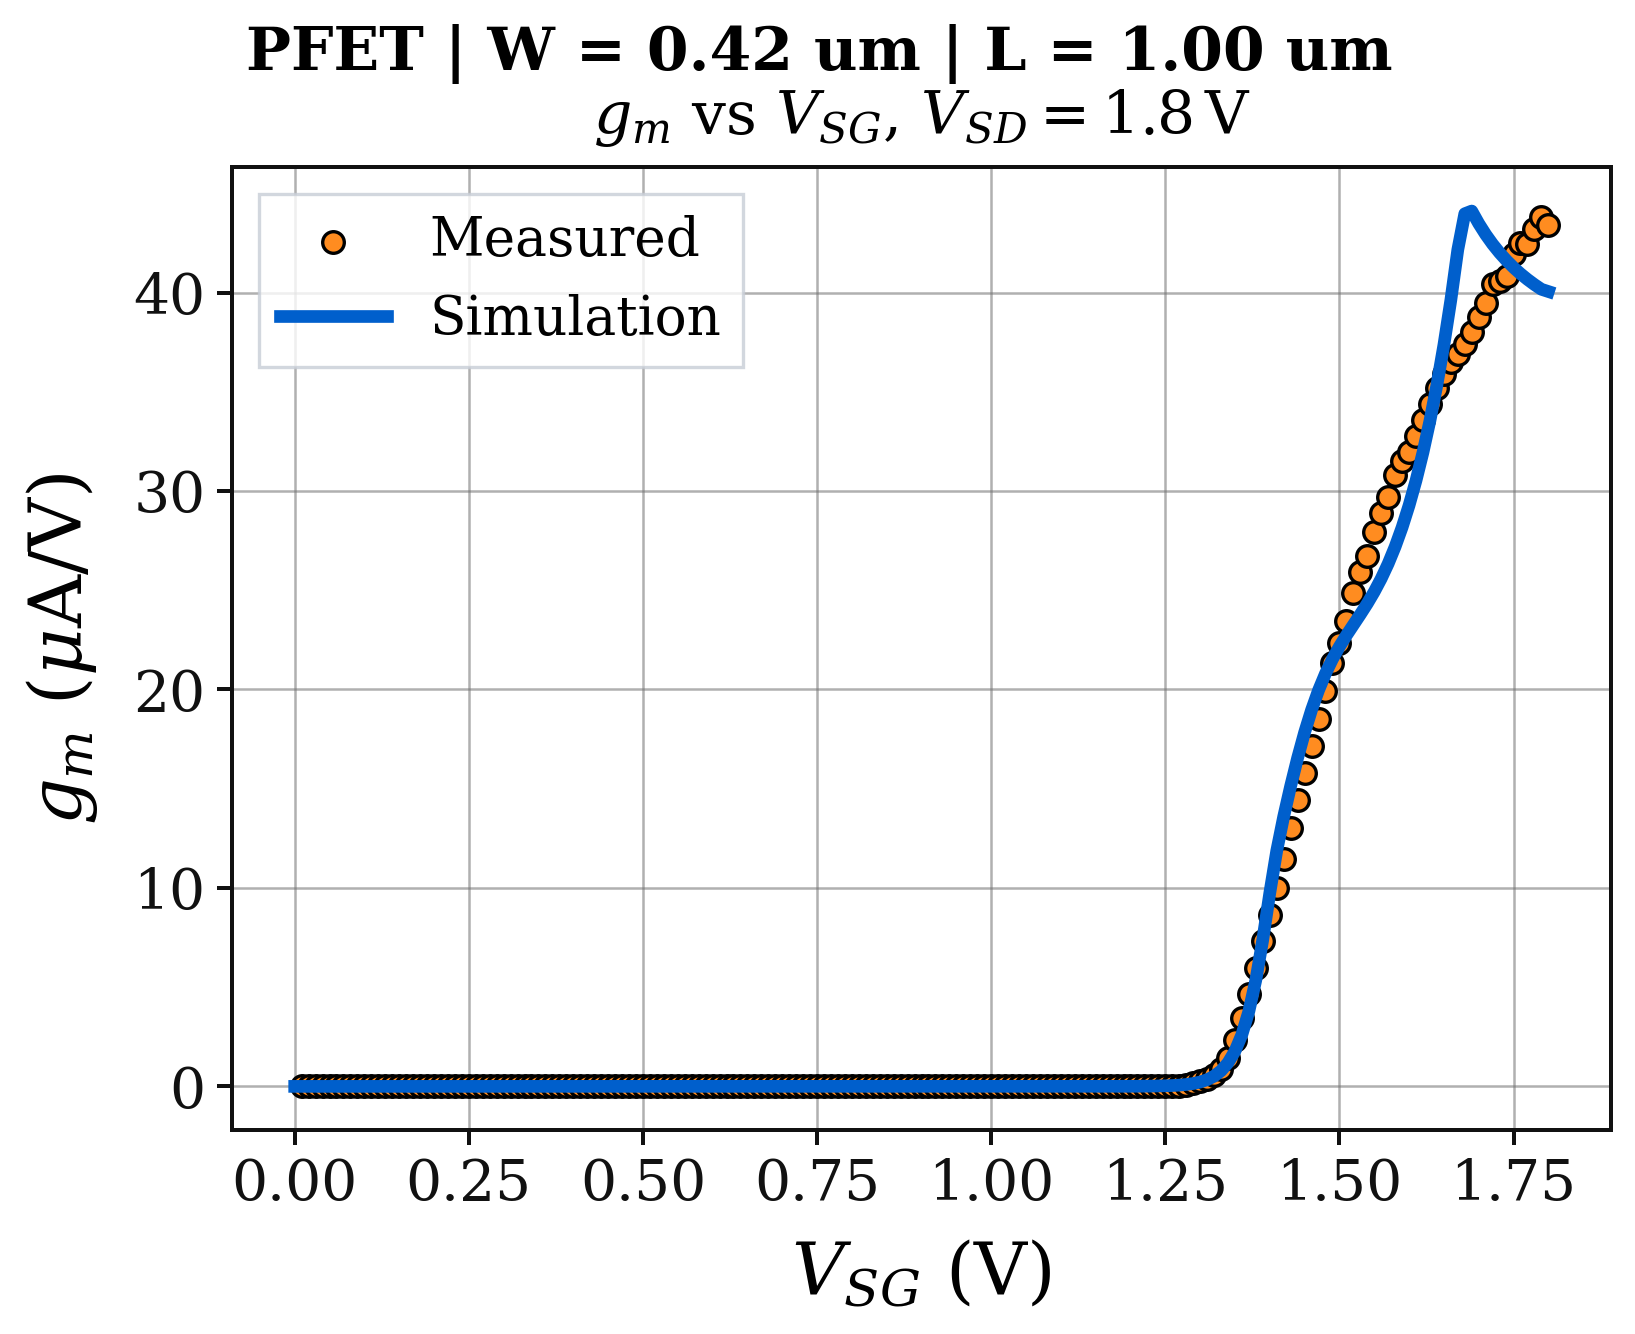
\includegraphics[width=\linewidth]{fig/publication_pfet_saturacao_w0p42_l1gmvg.png}\\
		{\tiny (b)}
	\end{minipage}

	\vspace{2mm}

	\begin{minipage}[t]{0.48\columnwidth}
		\centering
		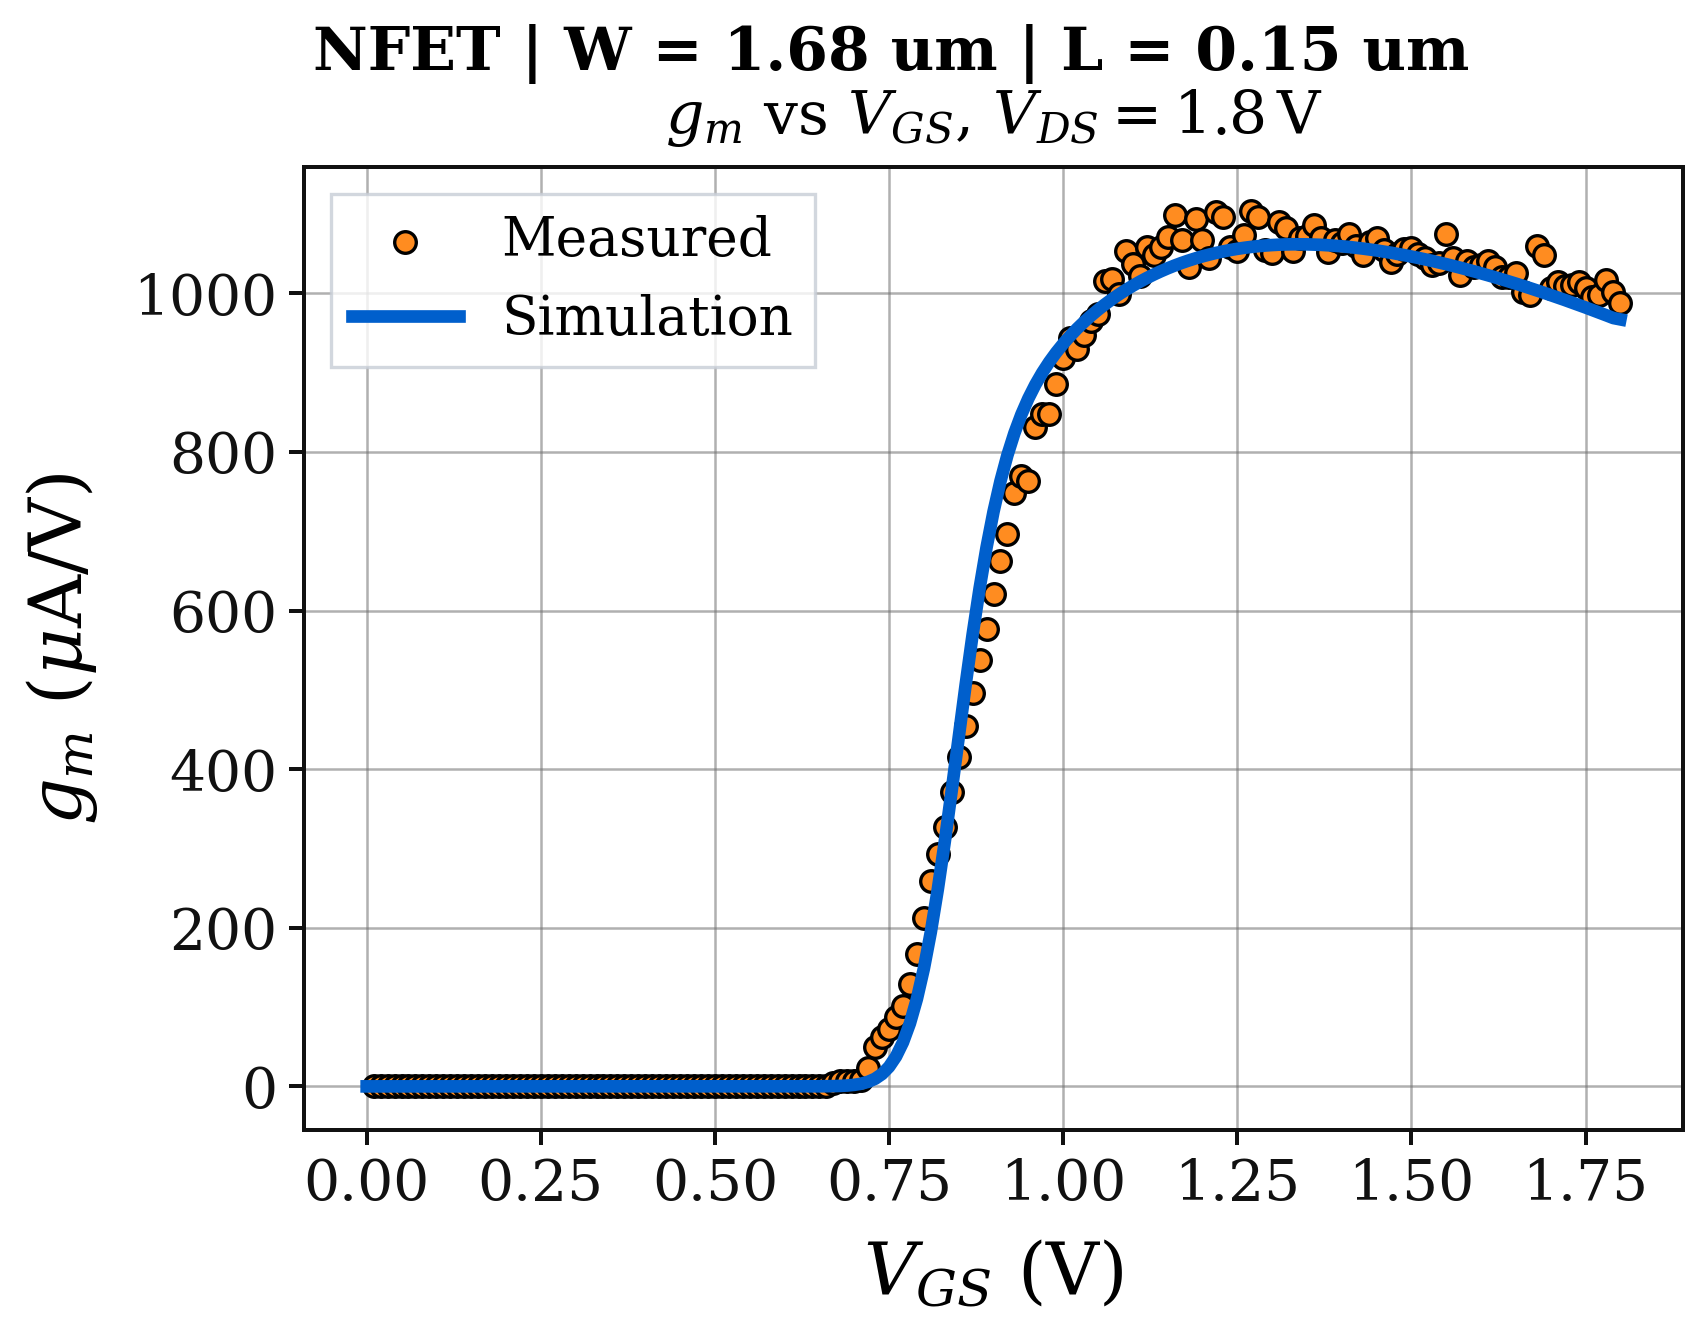
\includegraphics[width=\linewidth]{fig/publication_nfet_saturacao_w1p68_l0p15gmvg.png}\\
		{\tiny (c)}
	\end{minipage}
	\hfill
	\begin{minipage}[t]{0.48\columnwidth}
		\centering
		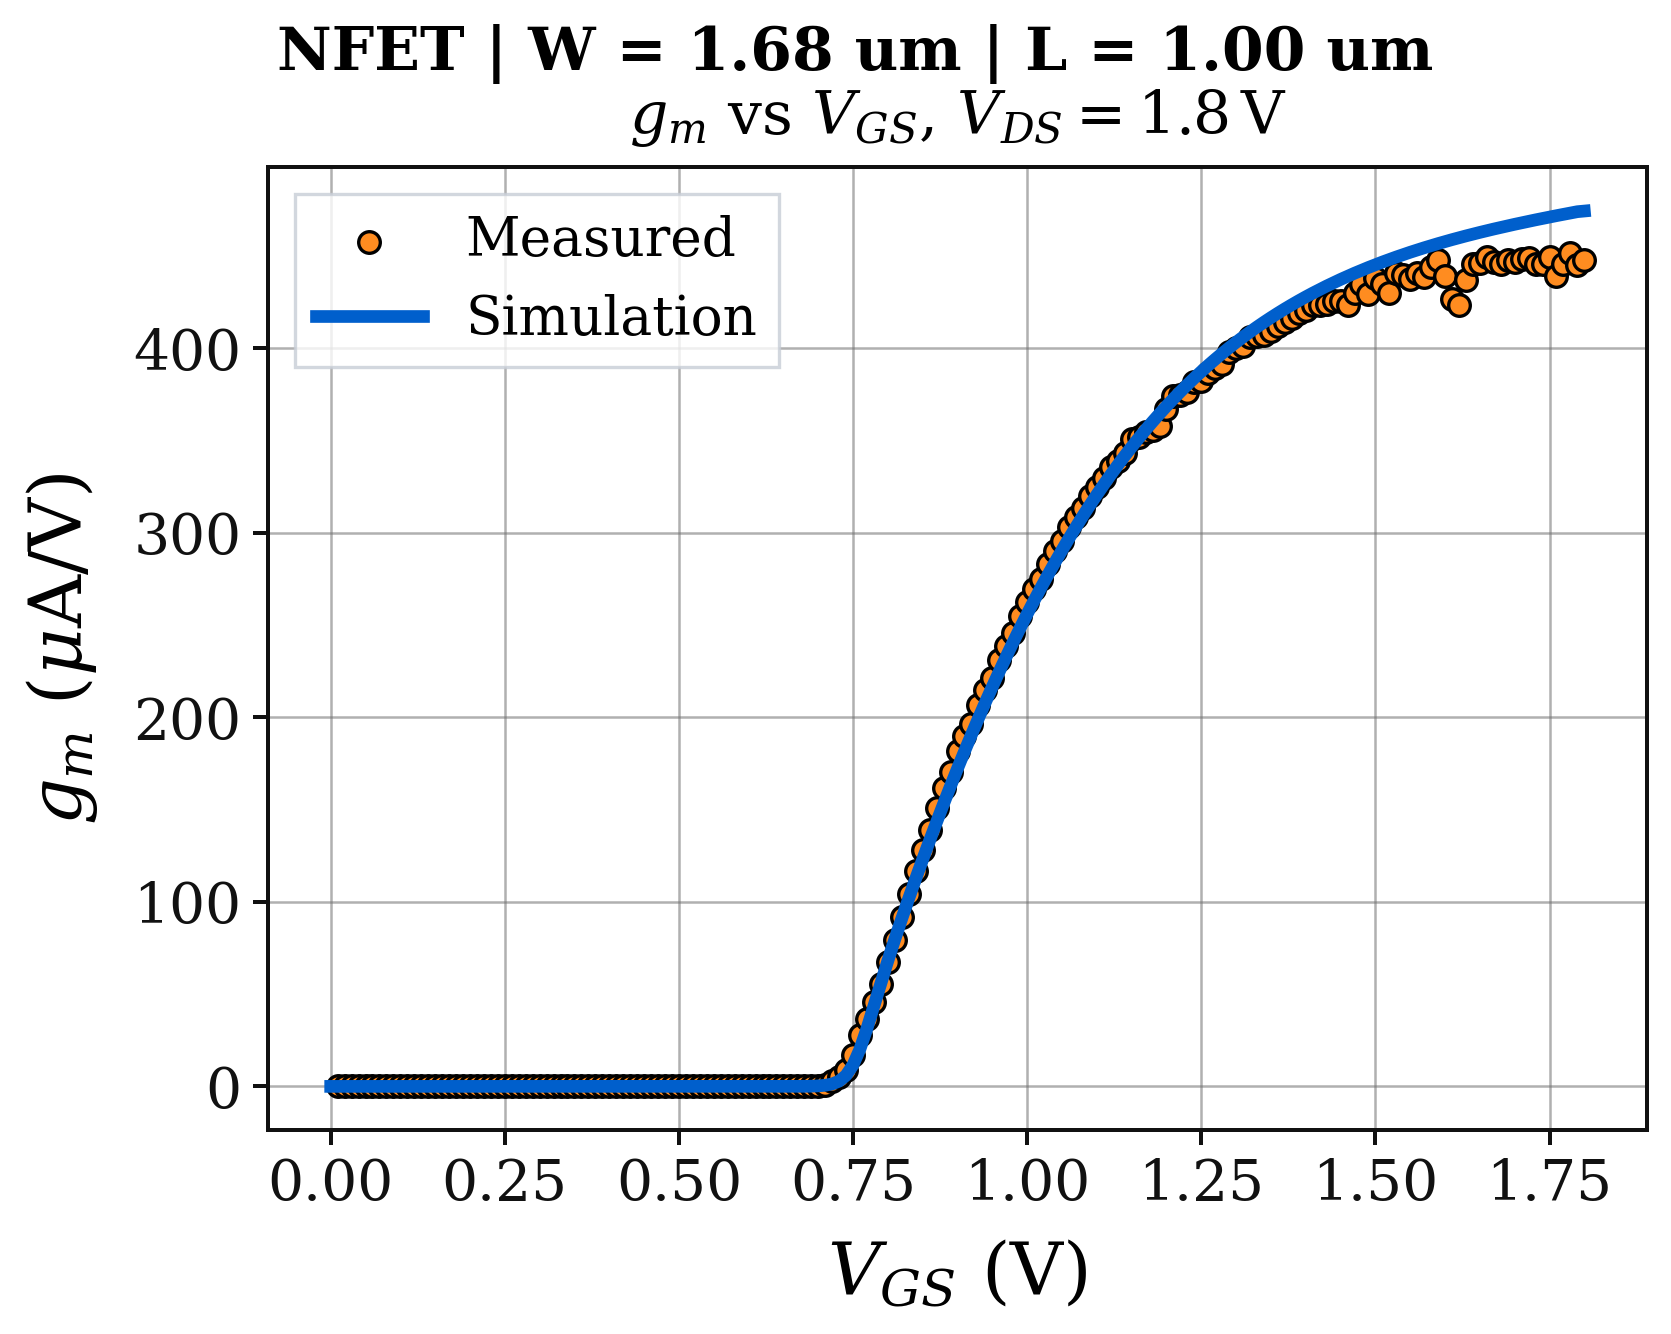
\includegraphics[width=\linewidth]{fig/publication_nfet_saturacao_w1p68_l1gmvg.png}\\
		{\tiny (d)}
	\end{minipage}
	\caption{Measured and simulated transconductance ($g_m$--$V_G$) characteristics for PFET and NFET devices at 4 K.}
	\label{fig:gmVG}
\end{figure}

Fig.~\ref{fig:gmID} shows the $g_m/I_D$ characteristics obtained for $V_{SD}=1.8\,\mathrm{V}$ (or $V_{DS}=1.8\,\mathrm{V}$ for NFET). Only data points with $I_{SD}>1\,\mathrm{pA}$ (or $I_{DS}>1\,\mathrm{pA}$ for NFET) are displayed, in order to exclude ultra-low-current regions where numerical convergence issues may arise in circuit simulation. Relative to the standard room-temperature Sky130 model, the calibrated 4 K model clearly reproduces the pronounced boost in $g_m/I_D$ in moderate inversion, in line with the cryogenic behavior reported in \cite{b4}.

\begin{figure}[h]
	\centering
	\begin{minipage}[t]{0.48\columnwidth}
		\centering
		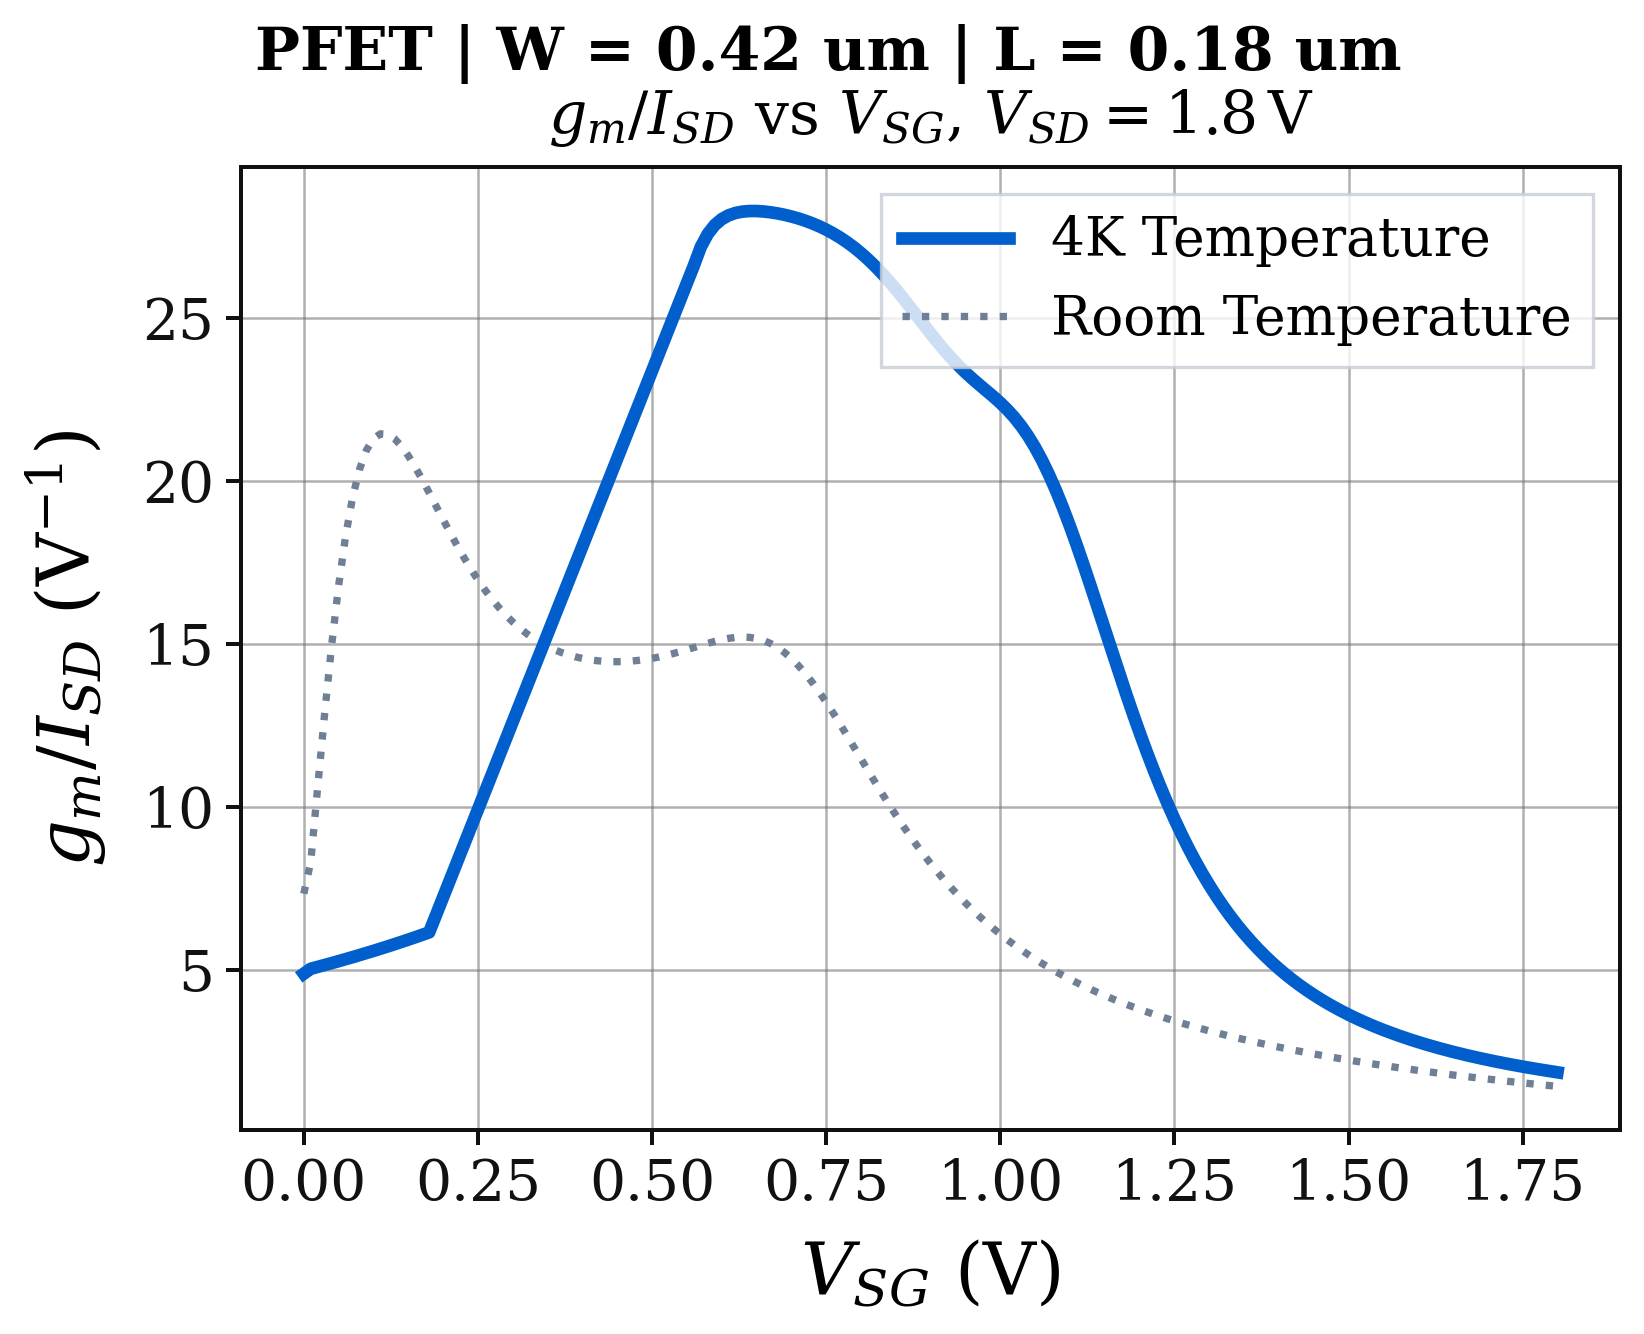
\includegraphics[width=\linewidth]{fig/publication_pfet_saturacao_w0p42_l0p18gmid.png}
	\end{minipage}
	\hfill
	\begin{minipage}[t]{0.48\columnwidth}
		\centering
		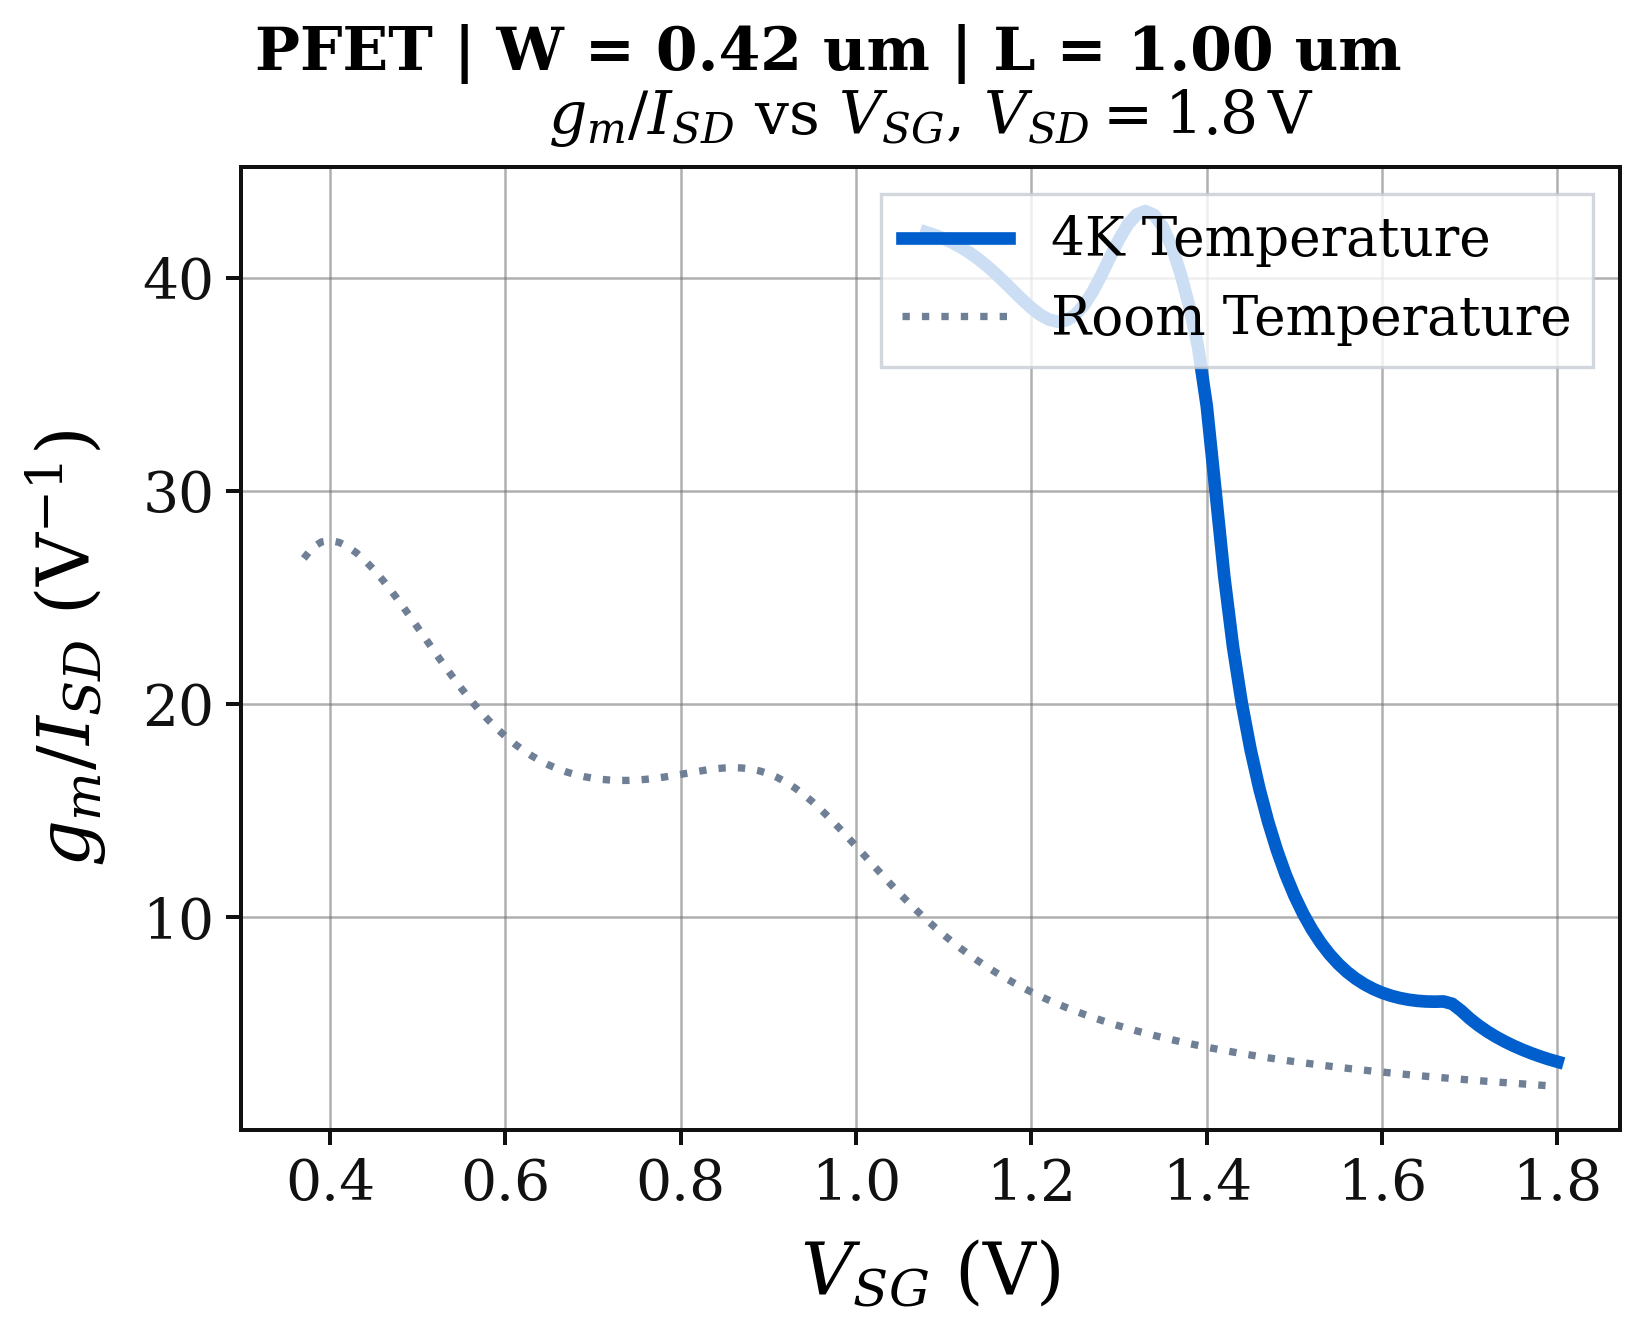
\includegraphics[width=\linewidth]{fig/publication_pfet_saturacao_w0p42_l1gmid.png}
	\end{minipage}

	\vspace{2mm}

	\begin{minipage}[t]{0.48\columnwidth}
		\centering
		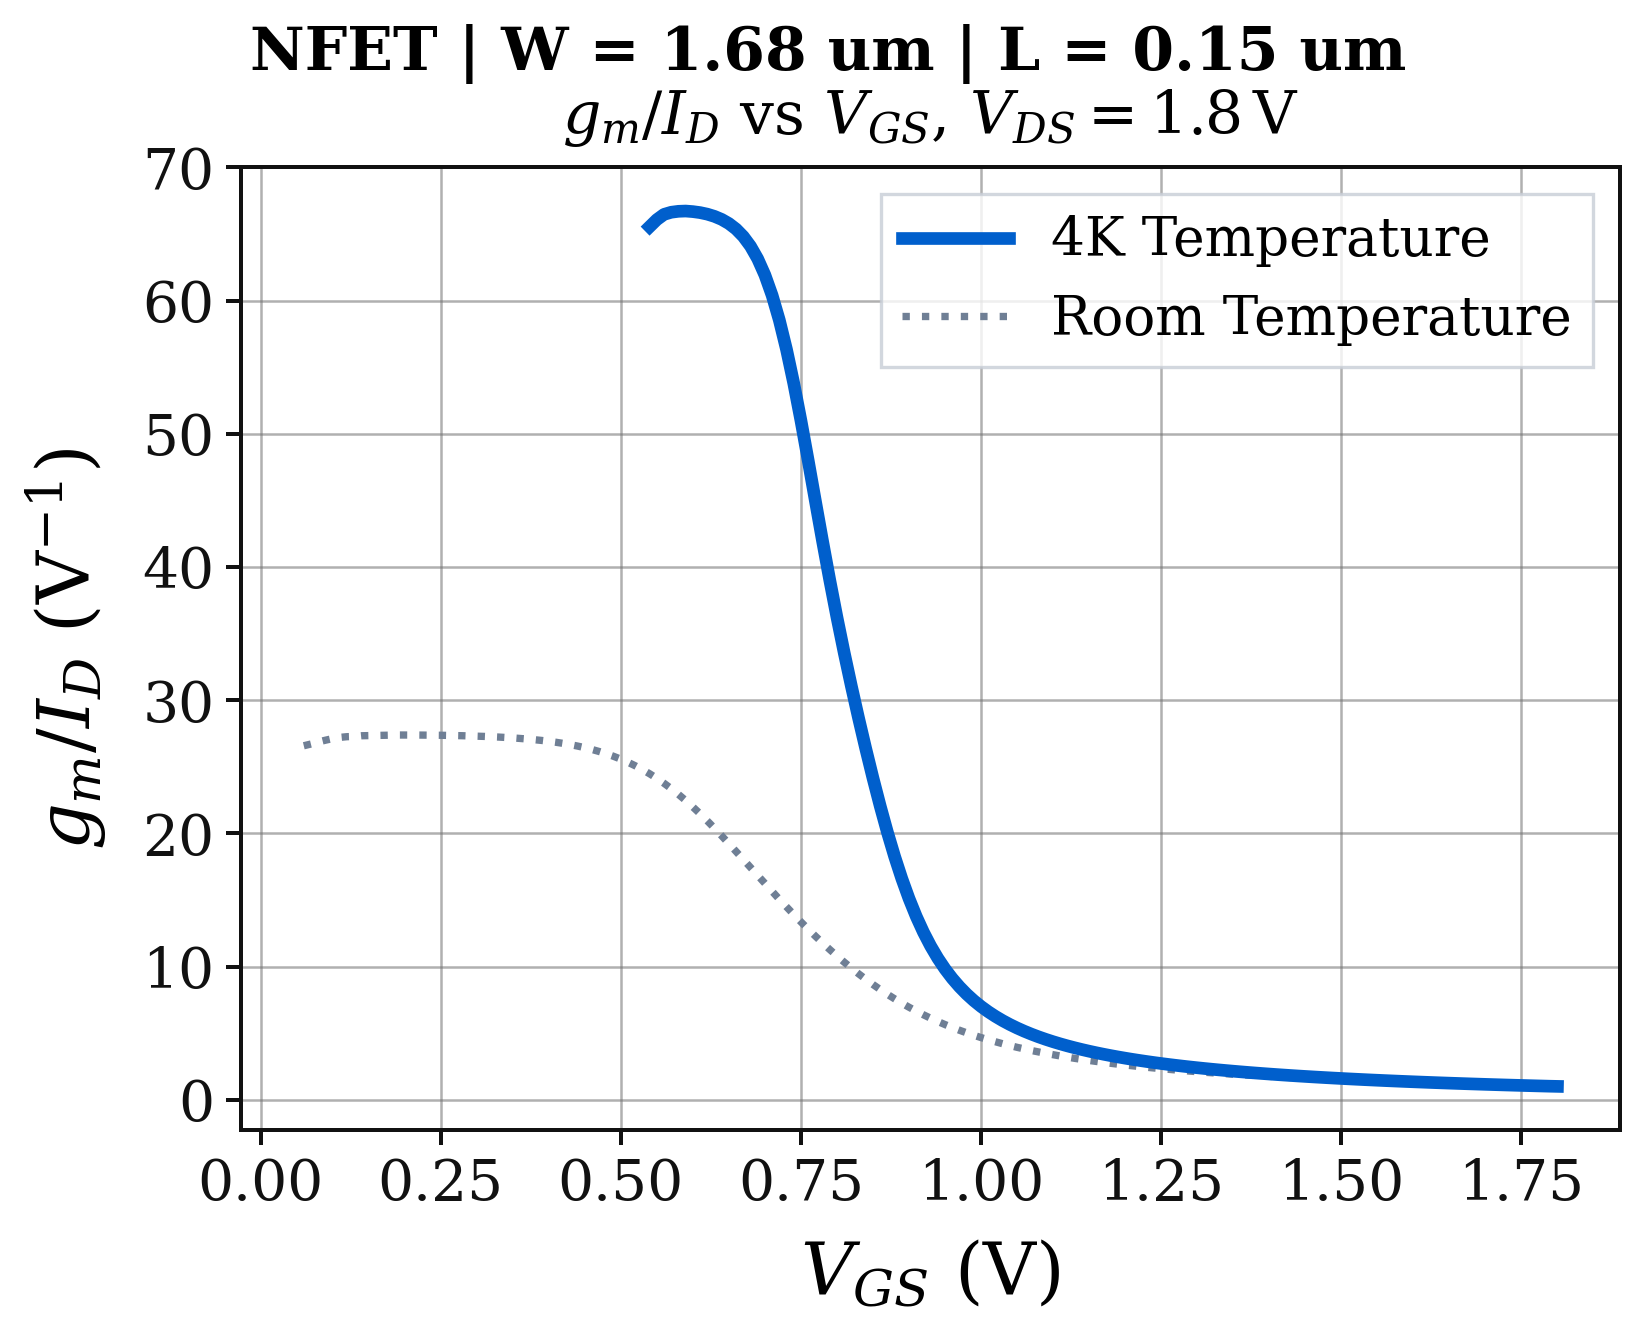
\includegraphics[width=\linewidth]{fig/publication_nfet_saturacao_w1p68_l0p15gmid.png}
	\end{minipage}
	\hfill
	\begin{minipage}[t]{0.48\columnwidth}
		\centering
		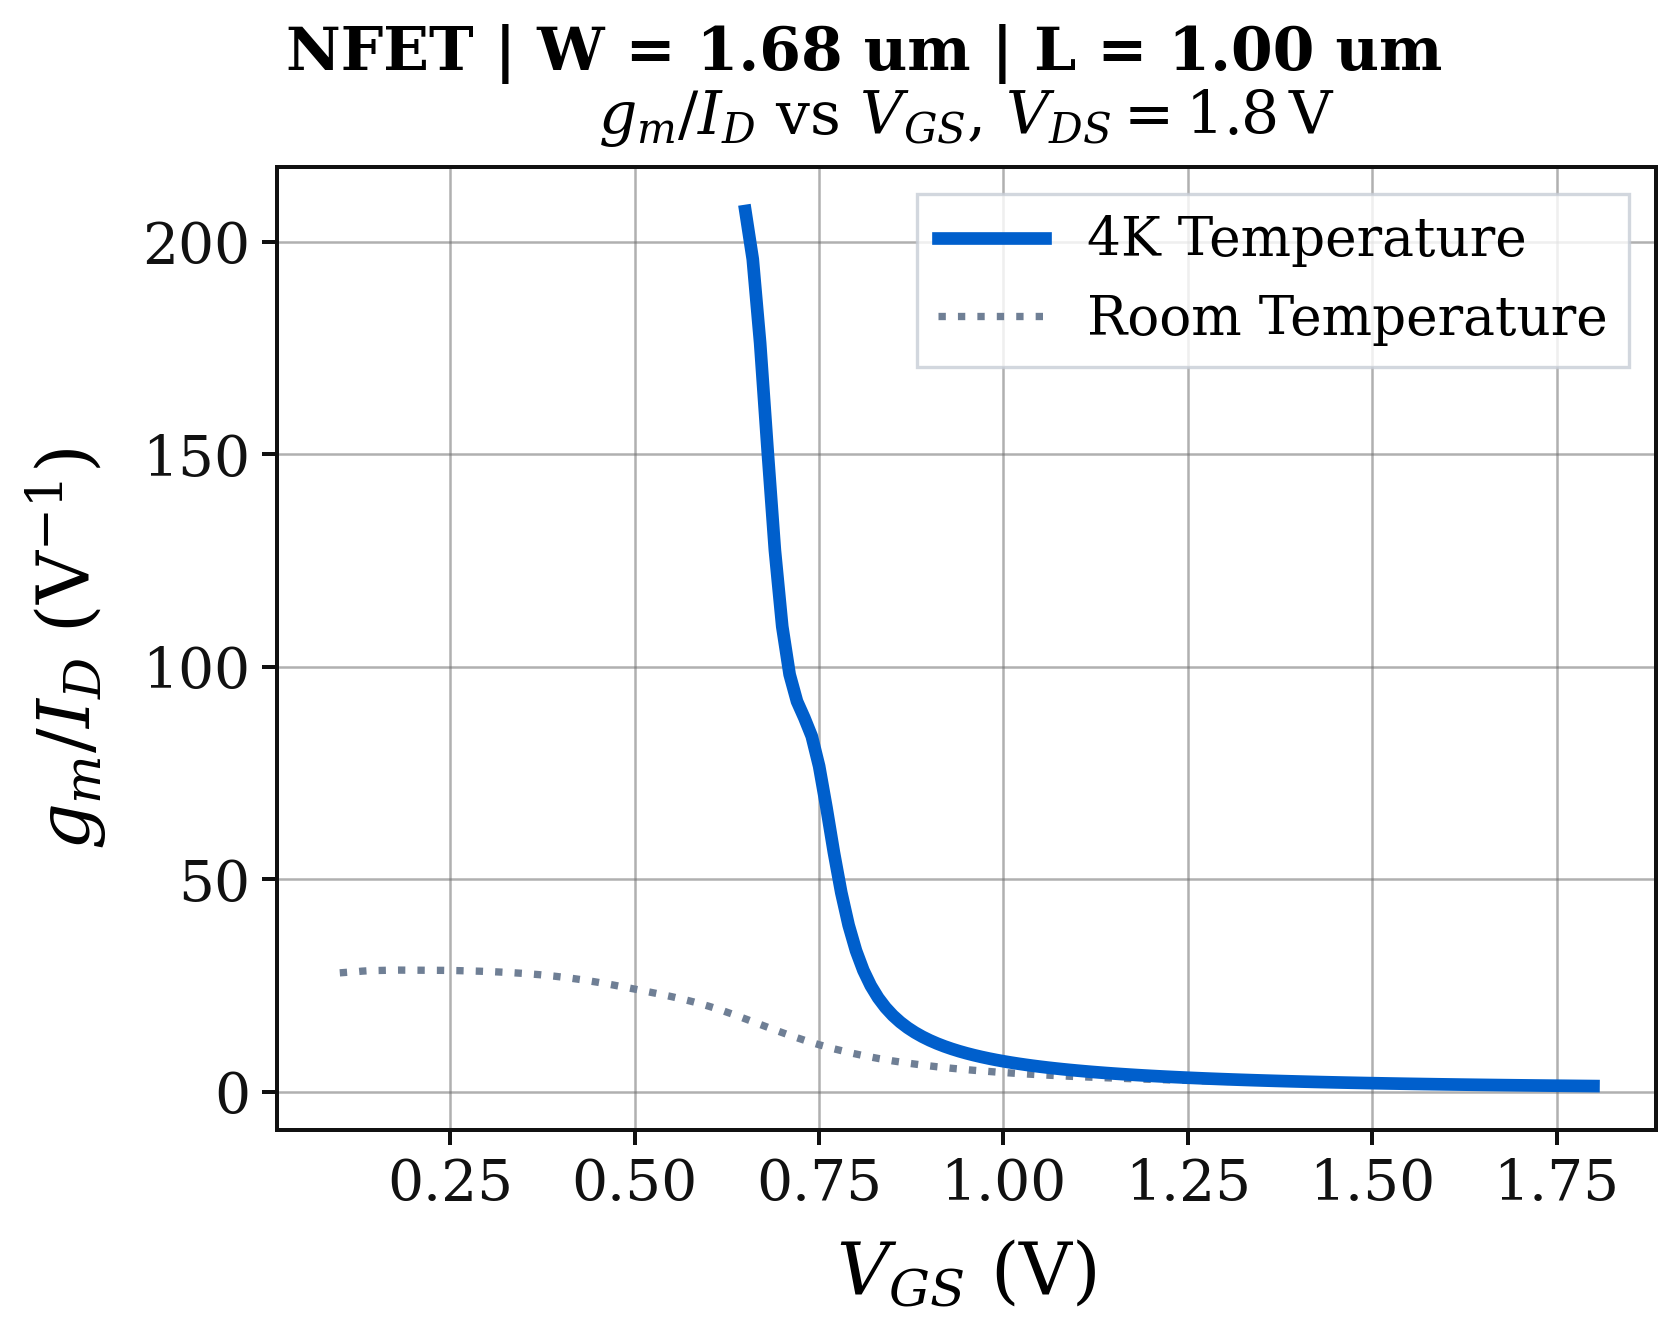
\includegraphics[width=\linewidth]{fig/publication_nfet_saturacao_w1p68_l1gmid.png}
	\end{minipage}
	\caption{$g_m/I_D$ characteristics obtained from simulation for PFET and NFET devices, comparing the standard Sky130 room-temperature model with the calibrated 4 K model. The results highlight the variation in transconductance efficiency under cryogenic operation for different channel lengths.}
	\label{fig:gmID}
\end{figure}

\subsection{Discussion}

Table~\ref{tab:comparison} summarizes the comparison with IceMOS \cite{b6}. The proposed methodology achieves competitive and, in some cases, lower errors in strong inversion. For the short-channel PMOS device, current and $g_m$ errors reached 0.42\% and 1.52\%, outperforming the IceMOS reference. NMOS current errors remained below 2.2\% for all evaluated geometries.

These results reflect the adopted calibration strategy, which prioritizes moderate and strong inversion, the most relevant region for analog and mixed-signal design. Larger discrepancies remain concentrated in weak inversion.

For comparison purposes, strong inversion was defined using $V_{OV}=150$ mV, a practical criterion widely used in analog design, although inversion level is more rigorously described by the inversion coefficient ($IC$) \cite{b14}. All values in Table~\ref{tab:comparison} were computed using this same criterion.

\begin{table}[htbp]\tiny
	\centering
	\caption{Comparison of mean relative error between the proposed calibrated model and IceMOS for drain current (\(I_D\)) and transconductance (\(g_m\)) at 4 K, considering PFET and NFET devices with different geometries.}
	\label{tab:comparison}
	\renewcommand{\arraystretch}{1.2}
	\begin{tabular}{|c|c|c|cc|}
		\hline
		\textbf{Device}                             & \textbf{Metric} & \textbf{IceMOS~\cite{b6}} & \multicolumn{2}{c|}{\textbf{This Work}}        \\ \hline
		\multirow{3}{*}{PFET}                       & W/L             & 0.42/0.15                 & \multicolumn{1}{c|}{0.42/0.18} & 0.42/1.00 \\ \cline{2-5}
		                                            & Current         & \pgfkeysvalueof{/erro_pmos_current/icemos}\%  & \multicolumn{1}{c|}{\pgfkeysvalueof{/erro_pmos_current/short}\%} & \pgfkeysvalueof{/erro_pmos_current/long}\%    \\ \cline{2-5}
		                                            & $g_m$           & \pgfkeysvalueof{/erro_pmos_gm/icemos}\%  & \multicolumn{1}{c|}{\pgfkeysvalueof{/erro_pmos_gm/short}\%}    & \pgfkeysvalueof{/erro_pmos_gm/long}\%    \\ \hline
		\multicolumn{1}{|l|}{\multirow{3}{*}{NFET}} & W/L             & 1.68/0.15                & \multicolumn{1}{c|}{1.68/0.15} & 1.68/1.00 \\ \cline{2-5}
		\multicolumn{1}{|l|}{}                      & Current         & \pgfkeysvalueof{/erro_nmos_current/icemos}\%  & \multicolumn{1}{c|}{\pgfkeysvalueof{/erro_nmos_current/short}\%}    & \pgfkeysvalueof{/erro_nmos_current/long}\%     \\ \cline{2-5}
		\multicolumn{1}{|l|}{}                      & $g_m$           & \pgfkeysvalueof{/erro_nmos_gm/icemos}\% & \multicolumn{1}{c|}{\pgfkeysvalueof{/erro_nmos_gm/short}\%}     & \pgfkeysvalueof{/erro_nmos_gm/long}\%     \\ \hline
	\end{tabular}
\end{table}

\section{Conclusion}

This work presented a fully automated methodology for generating cryogenic BSIM4 models for the Sky130 technology using experimental 4 K data. The proposed flow combines physics-based parameter initialization with iterative optimization, enabling scalable model extraction without manual parameter tuning.

The obtained results show that the methodology is particularly effective in the moderate-to-strong inversion region, where the calibrated models achieved satisfactory agreement with measured transfer, output, and transconductance characteristics. Since the optimization strategy prioritizes these operating regions, the resulting models are especially suitable for analog and mixed-signal designs that do not rely on weak-inversion operation.

Although larger discrepancies remain in deep-subthreshold conditions, the proposed models provide a practical and robust starting point for cryogenic circuit design in open-source technologies. In addition, the extracted parameter sets can also be used as initial seeds for further manual refinement in other calibration frameworks, such as IceMOS, significantly reducing calibration time and requiring only minor final adjustments.

Therefore, the proposed approach establishes an effective trade-off between automation, scalability, and design-oriented accuracy, contributing to faster and more accessible cryogenic model development for emerging applications such as quantum computing interfaces.
	% ACKNOWLEDGEMENTS SECTION
%\setcounter{secnumdepth}{0}
%\section{Acknowledgements}
%The authors would like to acknowledge...
	% BILIOGRAPHY SECTION
\bibliographystyle{IEEEtran}
\bibliography{IEEEabrv,article}
\end{document}
